\begin{savequote}[75mm]
The shortest path between two truths in the real domain passes through the complex domain.
\qauthor{--- Jacques Hadamard  ---}
\end{savequote}

\chapter{Methods of solution for first-order differential equations}
\label{First_Order_Quan}
\graphicspath{{figures/QuanFirst/}}

In this chapter we will study first-order differential equations for which there are general analytical methods of solution. We will start our investigation with linear first-order differential equations because these are the easiest to treat mathematically. Analytical solutions for their non-linear counterparts fall beyond the scope of this course. Instead, we will develop a few of the most important numerical methods for solving first-order differential equations.


\section{Linear first-order differential equations}
\label{seclineair}
\subsection{Existence and uniqueness of solutions}
A first-order differential equation is said to be  linear if it can be written in standard form as
\begin{equation}\label{eq:2.1.1}
y'+p(t)y=g(t)\,.
\end{equation}
A first-order differential equation that cannot be written like this is non-linear. In line with the terminology introduced in Section~\ref{naamgeving} we say that Equation~\eqref{eq:2.1.1} is homogeneous if $g\equiv0$; otherwise it is non-homogeneous. Since
$y(t)=0$ is obviously a solution of the homogeneous differential equation
$$
y'+p(t)y=0\,,
$$
we call it the \textbf{trivial solution} (\textit{triviale oplossing}). Any  other solution is non-trivial. 
\index{trivial solution}
\index{non-trivial solution}
\index[aut]{triviale oplossing}
\index[aut]{niet-triviale oplossing}
\index{homogeneous differential equation}
\index[aut]{homogene differentiaalvergelijking}
\index{non-homogeneous differential equation}
\index[aut]{inhomogene differentiaalvergelijking}
\index{linear differential equation}
\index[aut]{lineaire differentiaalvergelijking}


Before trying to find a solution of Equation~\eqref{eq:2.1.1}, it would be good to be assured that there exists a general solution, and given an initial condition $y(t_0)=y_0$, that there exists a unique solution of the initial value problem. For that purpose, the following theorem definitely helps.

\begin{theorem}[Existence and uniqueness theorem for linear first-order differential equations]
\label{theolineair}
Let the functions $p(t)$ and $g(t)$ be continuous on an open $t$-interval $\left.\right]a,b\left[\right.$ containing the point $t=t_0$, then there exists a unique function $y(t)$ that satisfies the differential equation
$$
y'+p(t)y=g(t),
$$
for every $t$ in $\left.\right]a,b\left[\right.$, and that also satisfies the initial condition $y\left(t_0\right)=y_0$.
\end{theorem}
\index{existence}
\index{uniqueness}
\index[aut]{bestaan}
\index[aut]{uniciteit}

In order to find the largest possible $t$-interval where Theorem~\ref{theolineair} guarantees that $y_{(t_0,y_0)}(t)$ is a unique solution of Equation~\eqref{eq:2.1.1} satisfying the initial condition $y\left(t_0\right)=y_0$, we merely have to look for the points $t$ where $p(t)$ and/or $g(t)$ are not continuous and choose the largest $t$-interval without any singularities  that contains $t_0$.

\begin{example}
Determine the largest possible $t$-interval where Theorem~\ref{theolineair} guarantees that $y_{(t_0,y_0)}(t)$ is a unique solution of the following differential equations:
\begin{enumerate}
	\item $2\,y'+t\,y=\sin(t)$,
	\item $y'+\dfrac{1}{t}\,y=0$,
	\item $\cos(t)\,y'+y=\sin(t)$,
\end{enumerate}
for $y(1)=y_0$.

\xhrulefill{gray}{2.5pt}Solution \xhrulefill{gray}{2.5pt}

\begin{enumerate}
	\item The functions $p(t)=t/2$ and $g(t)=\sin(t)/2$ are continuous everywhere, so this differential equation has a unique solution $y_{(1,y_0)}(t)$ on $\left.\right]-\infty,+\infty\left[\right.$.
	\item The function $p(t)=1/t$ is not continuous in $t=0$, while $g(t)=0$ is continuous everywhere $y'+\dfrac{1}{t}\,y=0$, so this differential equation has a unique solution $y_{(1,y_0)}(t)$ on $\left.\right]0,+\infty\left[\right.$.
	\item The functions $p(t)=1/\cos(t)$ and $g(t)=\sin(t)/\cos(t)=\tan(t)$  are not continuous in\\ $t=\pi/2+k\,\pi$, with $k\in\mathbb{Z}$, so this differential equation has a unique solution $y_{(1,y_0)}(t)$ on $\left.\right]-\pi/2,\pi/2\left[\right.$.
\end{enumerate}


\end{example}


\subsection{Homogeneous linear first-order differential equations}
\label{homolinsec}

Let us now try to find the general solution of the homogeneous linear first-order equation
$$
y'+p(t)y=0\,
$$
on $\left.\right]a,b\left[\right.$. 
We can rewrite this differential equation as 
\begin{equation}\label{eq:2.1.15}
\dfrac{y'}{y}=-p(t)
\end{equation}
for $t$ in $\left.\right]a,b\left[\right.$. Integrating both sides of Equation~\eqref{eq:2.1.15} yields 
\begin{equation}\label{eq:2.1.15.2}
\ln|y|=-\displaystyle\int p(t)\,d t + C'\,,
\end{equation}
where $C'$ is an integration constant. Upon introducing the antiderivative of $p(t)$, i.e.
$$
P(t)=\displaystyle\int p(t)\,d t\,,
$$
we can rewrite Equation~\eqref{eq:2.1.15.2} as
$$
\ln|y(t)|=-P(t) + C'\,.
$$

This implies that
$$
|y(t)|=e^{C'}\,e^{-P(t)}.
$$


Since a function that satisfies this equation cannot change sign on either $\left.\right]-\infty,0\left[\right.$ or $\left.\right]0,+\infty\left[\right.$ we can rewrite it as 
\begin{equation}
y(t)=C\,e^{-P(t)}\,,
\label{oplhomlin}
\end{equation}
 where
$$
C=\left\{\begin{array}{rcl}\phantom{-}e^{C'}, & \mbox{if} & y>0 \mbox{ on }
]a,b[, \\ -e^{C'}, &\mbox{if} & y<0\mbox{ on }]a,b[.\end{array}\right.
$$
Equation~\eqref{oplhomlin} is the general solution of a  homogeneous linear first-order differential equation. 

\begin{example}
Find the general solution of
\begin{equation}
 t\,y'+y=0.\label{eq:2.1.8}
\end{equation}
Then, determine the solution that satisfies $y(1)=3$ and the largest $t$-interval for which Theorem~\ref{theolineair} guarantees its uniqueness. 


\xhrulefill{gray}{2.5pt}Solution \xhrulefill{gray}{2.5pt}

First, we rewrite Equation~\eqref{eq:2.1.8} in standard form as
\begin{equation}\label{eq:2.1.10}
y'+\dfrac{1}{t}y=0.
\end{equation}
Hence, the function $p(t)$ is given by $1/t$, whose antiderivative equals
\begin{eqnarray*}
P(t)&=&\displaystyle\int p(t)\,d t\\
&=&\displaystyle\int\dfrac{1}{t} \, d t\\
&=&\ln|t|\,.
\end{eqnarray*}
So, substituting this expression for $P(t)$ in Equation~\eqref{oplhomlin}, we find the following general solution
\begin{equation}\label{eq:2.1.11}
y(t)=C\,e^{-\ln|t|}=\dfrac{C}{|t|}\,.
\end{equation}
Figure~\ref{ethomolin} shows some solution curves given by Equation~\eqref{eq:2.1.11} for varying values of the constant $C$, imposed on the direction field of Equation~\eqref{eq:2.1.8}. 
\begin{figure}[H]
	\begin{center}
			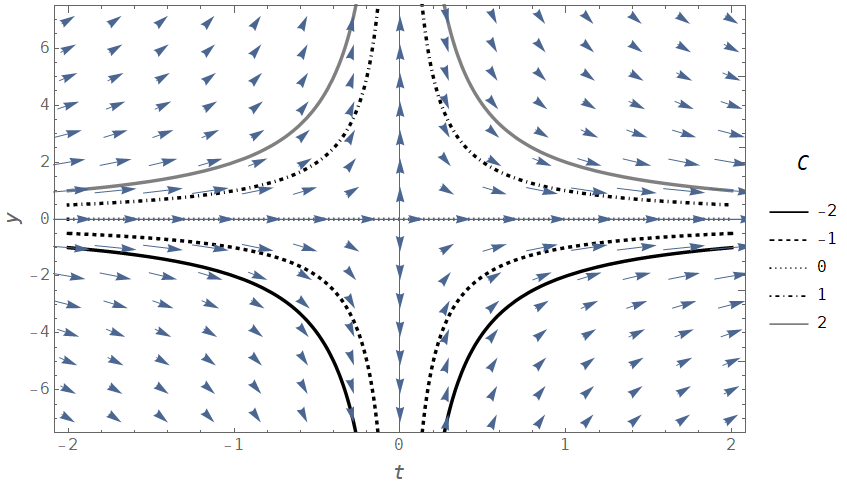
\includegraphics[width=0.6\textwidth]{exhomolin}
	\caption{Solution curves given by Equation~\eqref{eq:2.1.11} for varying values of the constant $C$, imposed on the direction field of Equation~\eqref{eq:2.1.8}.}
	\label{ethomolin}
	\end{center}
\end{figure}

Imposing the initial condition $y(1)=3$ on Equation~\eqref{eq:2.1.11} yields $C=3$. Therefore, the solution of the initial value problem defined by Equation~\eqref{eq:2.1.10} and $y(1)=3$ is
$$
y=\dfrac{3}{t}\,.
$$
Given the singularity of $p(t)$ in $t=0$, Theorem~\ref{theolineair} guarantees its uniqueness on  $\left.\right]0,+\infty\left[\right.$.

\end{example}

\subsection{Non-homogeneous linear first-order differential equations}

Here, we want to find the solution of the non-homogeneous linear first-order differential equation
\begin{equation}\label{eq:2.1.16}
y'+p(t)y=g(t)\,.
\end{equation}
Equation~\eqref{oplhomlin} is the general solution of its homogeneous counterpart, also referred to as the \textbf{complementary solution} (\textit{complementaire oplossing}) of the non-homogeneous differential equation $y_c(t)$. \index{complementary solution}\index[aut]{complementaire oplossing}

For solving Equation~\eqref{eq:2.1.16} let us assume that its general solution is the product of two functions, being an unknown function, say $u(t)$, and the complimentary solution $y_c(t)$. Essentially, we assume the following form for $y(t)$:
$$
y(t)=u(t)\,y_c(t)\,.
$$
Since $y=u\,y_c$ is assumed to be a solution of Equation~\eqref{eq:2.1.16}, the latter should still hold upon substituting $y=u\,y_c$ and its derivative, given by
$$
y'=u'\,y_c+u\,y_c'\,.
$$
Substituting these expressions for $y$ and $y'$ into Equation~\eqref{eq:2.1.16}
yields
$$
u'\,y_c+u\,(y_c'+p(t)\,y_c)=g(t)\,,
$$
which reduces to
\begin{equation}\label{eq:2.1.17}
u'\,y_c=g(t)\,,
\end{equation}
since $y_c(t)$ is a solution of the homogeneous equation; that is,
$$
y_c'+p(t)y_c=0\,.
$$
Given that $y_c=e^{-P(t)}$ has no zeros on an interval where $p(t)$ is continuous, we can divide Equation~\eqref{eq:2.1.17} by $y_c(t)$ to obtain
$$
u'=\dfrac{g(t)}{y_c(t)}=g(t)\,e^{P(t)}\,.
$$
Now, we can integrate this:
$$
u(t)=\displaystyle\int g(t)\,e^{P(t)} \, dt+C\,,
$$
where $C$ is an integration constant. Finally, we multiply the result by $y_c(t)$ to get the general solution of Equation~\eqref{eq:2.1.16}:
\begin{eqnarray}
y(t)&=&u(t)\,y_c(t)\nonumber\\
&=&y_c(t)\,\displaystyle\int g(t)\,e^{P(t)} \, dt+C\,y_c(t)\\\nonumber
&=&e^{-P(t)}\,\displaystyle\int g(t)\,e^{P(t)} \, dt + C\,e^{-P(t)}\,.
\end{eqnarray}
This result is summarized in the following theorem.

\begin{theorem}
\label{theolineairhetero}
Suppose  $p(t)$ and $g(t)$ are continuous on an open interval $\left.\right]a,b\left[\right.$. Then, the general solution of the non-homogeneous equation
\begin{equation}\label{eq:2.1.31}
y'+p(t)\,y=g(t)
\end{equation}
 on  $\left.\right]a,b\left[\right.$ is
\begin{equation}
y(t)=e^{-P(t)}\,\displaystyle\int g(t)\,e^{P(t)}\, dt+C\,e^{-P(t)}\,,
\label{oplheterolin}
\end{equation}
where $P(t)$ is the antiderivative of $p(t)$.
\end{theorem}

Of course, we must not know Equation~\eqref{oplheterolin} by heart to find the general solution of linear differential equation. Instead, we can just we can just follow the procedure leading to Theorem~\ref{theolineairhetero}.

\begin{example}\label{example:2.1.5}
Find the general solution of
\begin{equation}\label{eq:2.1.18}
y'+2y=t^3e^{-2t}.
\end{equation}

\xhrulefill{gray}{2.5pt}Solution \xhrulefill{gray}{2.5pt}

It is easy to see that $y_c(t)=C\,e^{-2t}$ is the complimentary solution of Equation~\eqref{eq:2.1.18}. Therefore we seek solutions of this differential equation in the form  $y(t)=u(t)\,e^{-2t}$. Since $y'=u'e^{-2t}-2\,u\,e^{-2t}$, we get after substituting $y$ and $y'$ in the left-hand side of Equation~\eqref{eq:2.1.18}:
\begin{eqnarray*}
y'+2\,y&=&u'e^{-2t}-2ue^{-2t}+2ue^{-2t}\,\\
&=&u'\,e^{-2t}\,.
\end{eqnarray*}
Therefore $y(t)$ is a solution of Equation~\eqref{eq:2.1.18} if and only if
$$
u'e^{-2t}=t^3e^{-2t} \,,
$$
or equivalently $u'=t^3$. Therefore
$$
u(t)=\dfrac{t^4}{4}+C\,,
$$
and
\begin{equation}
y(t)=u(t)\,e^{-2t}=e^{-2t}\left(\dfrac{t^4}{4}+C\right)
\label{eq:2.1.19}
\end{equation}
is the general  solution of Equation~\eqref{eq:2.1.18}.

Figure~\ref{etheterolin} shows some solution curves given by Equation~\eqref{eq:2.1.19} for varying values of the constant $C$ imposed on the direction field of Equation~\eqref{eq:2.1.18}. 

\begin{figure}[H]
	\begin{center}
			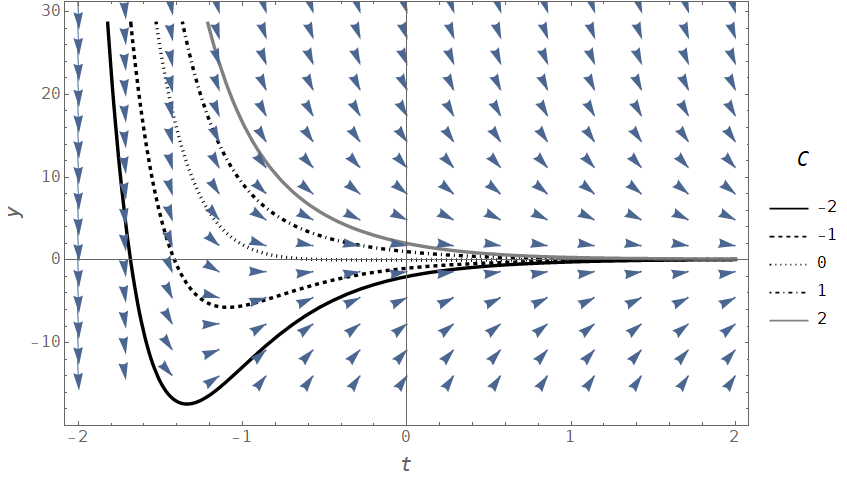
\includegraphics[width=0.6\textwidth]{exheterolin}
	\caption{Solution curves given by Equation~\eqref{eq:2.1.19} for varying values of the constant $C$ imposed on the direction field of Equation~\eqref{eq:2.1.18}.}
	\label{etheterolin}
	\end{center}
\end{figure}


\end{example}

\begin{example}
To conclude, we will try to find the general solution of the differential equation describing the velocity of a free-falling object (Equation~\eqref{freefall3}):
$$
m\,v'=m\,g-\mu\,v\,.
$$
We start by rewriting it in standard form, i.e.
$$
v'+\dfrac{\mu\,v}{m}=g\,,
$$
from which we infer that both $p(t)=\mu/m$ and $g(t)=g$ are constant. So, $P(t)=\frac{\mu}{m}\,t$ and the complimentary solution is given by $y_c(t)=e^{-\frac{\mu}{m}\,t}$. Direct application of Equation~\eqref{oplheterolin} yields
$$
v(t)=e^{-\frac{\mu}{m}t}\,\displaystyle\int g\,e^{\frac{\mu}{m}t}d t+C\,e^{-\frac{\mu}{m}t}\,,
$$
which after evaluating the integral can be simplified to
$$
v(t)=\frac{g\,m}{\mu}+C\,e^{-\frac{\mu}{m}t}\,.
$$
This general solution clearly shows that 
$$
\lim_{t\to+\infty}v(t)=\dfrac{g\,m}{\mu}\,,
$$
which corroborates our findings in Section~\ref{equipoints}, for what concerns the terminal velocity of the free-falling object. Some solution curves are illustrated in Figure~\ref{FreeFallDF2}, together with the corresponding direction field. 

\end{example}


Even though linear differential equations are intrinsically simple, they are useful to describe phenomena governed by a first-order kinetics, where the rate by which a certain compound reacts is proportional to the mass or concentration of that component. In the next example, we will study one such a process in more detail. 

\begin{example}\label{exampletank}
Consider a waste water treatment plant where waste water is circulated in huge aerated cylindrical tanks so that microorganisms are stimulated to decompose to organic material present in the waste water. Figure~\ref{TankEcht} shows such a typical tank, while its schematic representation is depicted in Figure~\ref{Tank}. At the top of the tank with volume $V$ [L$^3$] waste water enters the tank with a constant flow rate $q$ [L$^3$\,T$^{-1}$]. The known concentration of the organic material in this influent is $C_{in}$ [M\,L$^{-3}$]. Water leaves the tank at the bottom with a flow rate $q$ [L$^3$\,T$^{-1}$] and concentration  $C_{out}$ [M\,L$^{-3}$]. Microorganisms decompose the organic material in the tank with a rate constant $r$ [T$^{-1}$]. In the centre of the tank there is a paddle that ensures that the fluid is well mixed. 

\begin{figure}[H]
\centering
%\raisebot{0.5cm}{
\centerline{
\subfigure[\label{TankEcht}]{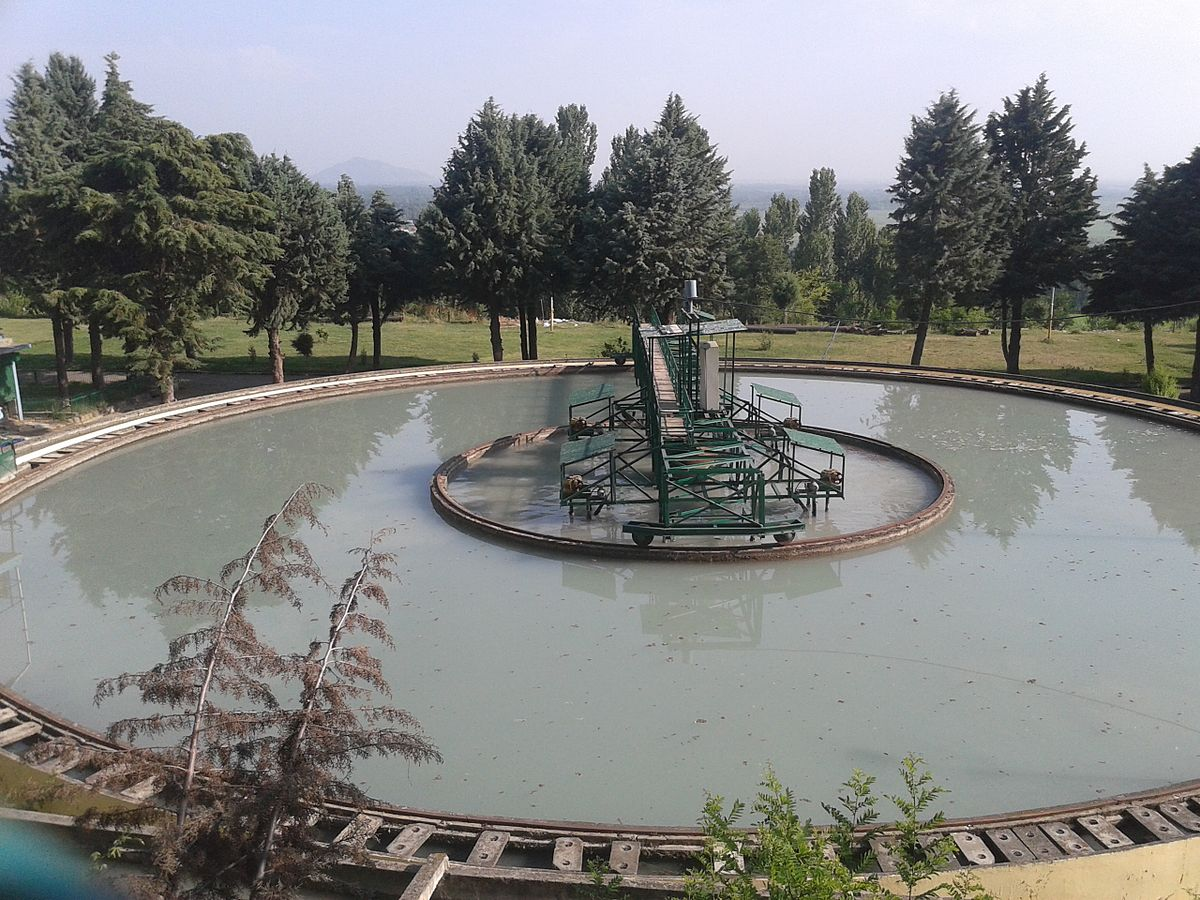
\includegraphics[width=0.49\textwidth]{TankEcht}}
\hspace{0.1cm}
\subfigure[\label{Tank}]{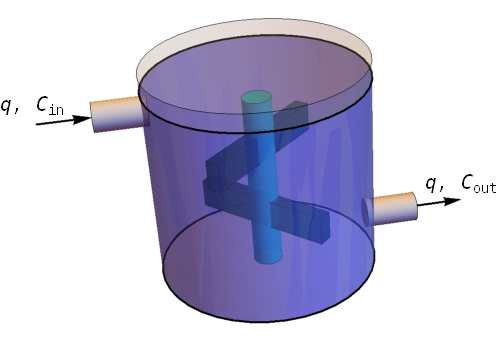
\includegraphics[width=0.49\textwidth]{Tank}}
}
\caption{A typical aeration tank of a waste water treatment plant (a) and its schematic representation (b).} 

\end{figure}

In operation phase, we normally want to know how long it takes before the concentration of organic material in the tank gets lower than a certain threshold, as this guarantees the quality of the effluent. So, we want to find how the concentration $C(t)$ in the tank changes over time. For that purpose, let us try to formulate a mass balance equation for the organic material (OM) in the tank, based on the law of mass conservation. Since OM cannot just disappear, it should hold that:


\[
	\left.\begin{array}{c}
    \mbox{Change of mass}\\
	\mbox{OM in tank }\\
	\mbox{during $\Delta t$}
	\end{array}
	\right. =
	\left.\begin{array}{c}
	\mbox{Mass OM }\\
    \mbox{entering tank}\\
	\mbox{during $\Delta t$}
	\end{array}
	\right. -
	\left.\begin{array}{c}
	\mbox{Mass OM }\\
    \mbox{leaving tank }\\
	\mbox{during $\Delta t$}
	\end{array}
	\right.
	-
	\left.\begin{array}{c}
	\mbox{Mass OM decomposed}\\
    \mbox{by microorganisms}\\
	\mbox{during $\Delta t$}
	\end{array}
	\right.
\]

The mass $M$ entering the tank during $\Delta t$ is given by
$$
q\,C_{in}\,\Delta t\,,
$$
and similarly the mass leaving the tank during $\Delta t$ is given by
$$
q\,C_{out}\,\Delta t\,. 
$$
Now, we face the problem that $C_{out}$ is not known. Yet, at this point we can rely on the fact that the tank is well mixed, meaning that the concentration in tank is spatially homogeneous. Consequently, the concentration in the effluent is the same as the concentration in tank, i.e.
$$
q\,C_{out}\,\Delta t=q\,C\,\Delta t\,. 
$$
The last term that we need to formalize in the mass balance equation is the one relating to the decomposition of the organic material by the micro-organisms. If we assume that this decomposition is proportional to the concentration of organic material in the tank (first-order kinetics), we get 
$$
r\,C\,\,V\Delta t\,.
$$
Plugging these expression into the mass balance equation, we obtain:
$$
\Delta M=q\,C_{in}\,\Delta t-q\,C\,\Delta t-r\,C\,\,V\Delta t\,,
$$
or since $C=M/V$, in terms of the concentration of organic material:
$$
\Delta C=\dfrac{q\,C_{in}\,\Delta t}{V}-\dfrac{q\,C\,\Delta t}{V}-r\,C\,\Delta t\,.
$$
We can also express the concentration change per unit of time by dividing both sides by $\Delta t$:
\begin{equation}
\label{eentankDE}
\dfrac{\Delta C}{\Delta t}=\dfrac{q\,C_{in}}{V}-\dfrac{q\,C}{V}-r\,C\,.
\end{equation}
Finally, we assume that $\Delta t$ becomes infinitesimally small, so $\Delta M$ too, and we arrive at the continuum limit of Equation~\eqref{eentankDE}:
$$
C'=\dfrac{q\,C_{in}}{V}-\dfrac{q\,C}{V}-r\,C\,.
$$
This is a linear first-order differential equation, which reads in standard form:
\begin{equation}
\label{eentank}
C'+\left(\dfrac{q}{V}+r\right)C=\dfrac{q\,C_{in}}{V}\,.
\end{equation}
We leave a detailed analyse of this equation and the behaviour of its solutions to the exercises. 
\end{example}

\pagebreak

\section{Solutions of non-linear first-order differential equations}
Before turning to the method for solving first-order differential equations, we will first state the existence and uniqueness theorem for non-linear first-order differential equations. 

\begin{theorem}[Existence and uniqueness theorem for non-linear first-order differential equations]
\label{theononlineair}
\begin{enumerate}
\item If  $f$ is a continuous function on an open rectangle
$$
R:  \{ a < t < b, c < y < d \}
$$
 that contains $(t_0,y_0)$, then  the initial value problem
\begin{equation} \label{eq:2.3.1}
y'=f(t,y), \quad y(t_0)=y_0
\end{equation}
 has at least one solution  on some open subinterval of  $\left.\right]a,b\left[\right.$ that contains $t_0$. 

\item  If  both $f$ and  $f_y = \frac{\partial f}{\partial y}$ are  continuous on $R$, then the initial value problem~\eqref{eq:2.3.1} has a unique solution on some open subinterval  of $\left.\right]a,b\left[\right.$ that contains $t_0$.
\end{enumerate}
\end{theorem}


It is important to understand exactly what Theorem~\ref{theononlineair} means. Its first part guarantees that a solution exists on some open $t$-interval that contains $t_0$, but provides no information on how to find the solution, or to determine the open $t$-interval on which it exists. Moreover, it provides no information on the number of solutions that the initial value problem \eqref{eq:2.3.1} may have. It leaves open the possibility that it has two or more solutions that differ for values of $t$ arbitrarily close to $t_0$. The second part of Theorem~\ref{theononlineair} guarantees that the initial value problem \eqref{eq:2.3.1} has a unique solution on some open subinterval of $\left.\right]a,b\left[\right.$ that contains $t_0$. 

\begin{example}\label{example:2.3.2}
Consider the differential equation
\begin{equation} \label{eq:2.3.4}
y'=\dfrac{t^2-y^2}{t^2+y^2}\,,
\end{equation}
subject to $y(t_0)=y_0$.

The right-hand side of Equation~\eqref{eq:2.3.4} is given by
$$
f(t,y)  =  \dfrac{t^2-y^2}{t^2+y^2}\,,
$$
and its derivative with respect to $y$ by
$$
f_y(t,y)  =  -\dfrac{4\,t^2\,y}{(t^2+y^2)^2}\,.
$$
Both are continuous everywhere, except at $(0,0)$. If $(t_0,y_0) \ne(0,0)$, there is  an open rectangle $R$ that contains
$(t_0,y_0)$ that does not contain $(0,0)$ and where $f$ is continuous. This already implies that Equation~\eqref{eq:2.2.4} has at least one solution on some open $t$-interval that contains $t_0$. Moreover, since $f$ and $f_y$ are continuous on $R$, Theorem~\ref{theononlineair} implies that if
$(t_0,y_0)\ne(0,0)$, then the initial value problem has a unique solution on some open $t$-interval $]a,b[$ that contains $t_0$.
\end{example}

\begin{example}\label{example:2.3.5}
\rm  Consider the initial value problem
\begin{equation} \label{eq:2.3.8}
y' = {10\over 3}ty^{2/5}, \quad y(t_0) = y_0.
\end{equation}
\begin{enumerate}
\item For what points $(t_0,y_0)$ does Theorem~\ref{theononlineair} imply that it has a solution?
\item For what points $(t_0,y_0)$ does Theorem~\ref{theononlineair} imply that it has a unique solution on some open $t$-interval that contains $t_0$?
\end{enumerate}

\xhrulefill{gray}{2.5pt}Solution \xhrulefill{gray}{2.5pt}

\begin{enumerate}
\item Since
$$
f(t,y) = \dfrac{10}{ 3}t\,y^{2/5}
$$
is continuous for all $(t,y)$,  Theorem~\ref{theononlineair} implies that the initial value problem \eqref{eq:2.3.8} has at least one solution for every $(t_0,y_0)$.

\item Here, we have that
$$
f_y(t,y) = \dfrac{4}{3}t\,y^{-3/5}
$$
is continuous for all $(t,y)$, except where $y_0=0$. Therefore, if $y_0\ne0$ there is an open rectangle $R$ on which both $f$ and $f_y$ are continuous, and Theorem~\ref{theononlineair} implies that the initial value problem~\eqref{eq:2.3.8} has
a unique solution on some open interval that contains $t_0$. If $y=0$ then $f_y(t,y)$ is discontinuous;
hence, Theorem~\ref{theononlineair} does not apply to the initial value problem~\eqref{eq:2.3.8} if $y_0=0$.
\end{enumerate}
\end{example}


At this point, it is important to realize the difference between linear and non-linear first-order differential equations in terms of the existence and uniqueness guaranteed by Theorem~\ref{theolineair} and \ref{theononlineair} respectively.  The former states that if $p(t)$ and $g(t)$ are continuous on $\left.\right]a,b\left[\right.$ then the solution of
$$
y'+p(t)\,y=g(t)
$$
satisfying $y(t_0)=y_0$ is guaranteed to exist on the entire open interval $\left.\right]a,b\left[\right.$ and is the only one on $\left.\right]a,b\left[\right.$. This is, however, not true for non-linear first-order differential equations. Indeed, Theorem~\ref{theononlineair} merely assures that there is at least one solution on some open subinterval of $\left.\right]a,b\left[\right.$ if $f$ is continuous on some open rectangle $R$ containing $(t_0,y_0)$. Besides, it only assures its uniqueness on this subinterval if also  $f_y$ is continuous on  $R$. Still, both theorems imply that two solutions cannot intersect in a point where their premises are fulfilled. 

\section{Separable differential equations}

A first-order differential equation is \textbf{separable} (\textit{scheidbaar}) if it can be written as
\begin{equation} \label{eq:2.2.1}
h(y)y'=g(t),
\end{equation}
where the left side is a product of $y'$ and a function of $y$ and the right side is a function of $t$ only. Rewriting a separable
differential equation in this form is called \textbf{separation of variables} (\textit{scheiding van veranderlijken}). Essentially, without really giving it a name we already used separation of variables to solve homogeneous linear differential equations in Section~\ref{homolinsec}. Here we will apply this method to non-linear differential equations. \index{separable differential equations} \index[aut]{Scheidbare differentiaalvergelijkingen} \index{separation of variables} \index[aut]{scheiden van veranderlijken}

To see how to solve Equation~\eqref{eq:2.2.1}, let us first assume that $y(t)$ is a solution. Moreover, let  $H(t)$ and $G(y)$ be antiderivatives of $h(y)$ and $g(t)$, respectively; that is,
\begin{equation} \label{eq:2.2.2}
H(y)=\displaystyle\int h(y) \, d y\mbox{\quad and \quad} G(t)=\displaystyle\int g(t) \, d t\,.
\end{equation}
Then, using the fact that $y'=d y/d t$, we may rewrite Equation~\eqref{eq:2.2.1} as
$$
h(y)\,d y=g(t)\,d t\,,
$$
so that we can integrate both sides
$$
\displaystyle\int h(y) \,d y=\displaystyle\int g(t) \,d t
$$
to obtain
\begin{equation} \label{eq:2.2.3}
H(y(t))=G(t)+C\,,
\end{equation}
where $C$ is an integration constant. 

Although we derived this equation on the assumption that $y(t)$ is a solution of Equation~\eqref{eq:2.2.1}, we can now view it differently. Any differentiable function $y$ that satisfies Equation~\eqref{eq:2.2.3} for some constant $C$ is a solution of Equation~\eqref{eq:2.2.1}. To see this, we differentiate both sides of Equation~\eqref{eq:2.2.3} with respect to $t$, using the chain rule on the left, to obtain
$$
H'(y(t))y'(t)=G'(t)\,,
$$
which is equivalent to
$$
h(y(t))y'(t)=g(t)
$$
because of Equations~\eqref{eq:2.2.2}.

In conclusion, to solve Equation~\eqref{eq:2.2.1} it suffices to find functions $G=G(t)$ and $H=H(y)$ that satisfy Equations~\eqref{eq:2.2.2}. Then any differentiable function  $y=y(t)$  that satisfies Equation~\eqref{eq:2.2.3} is a solution of Equation~\eqref{eq:2.2.1}.


\begin{example}\label{example:2.2.1}
Solve the following first-order differential equation:
$$
y'=t\left(1+y^2\right).
$$

\xhrulefill{gray}{2.5pt}Solution \xhrulefill{gray}{2.5pt}


Separating variables yields
$$
\dfrac{y'}{1+y^2}=t\,.
$$
Integrating yields
$$
\arctan (y)=\dfrac{t^2}{2}+C.
$$
Therefore
$$
y(t)=\tan\left({t^2\over2}+C\right).
$$
\vspace*{-0.5cm}
\end{example}

There are many situations where one ends up with an implicit solution of the differential equation when using the method of separation of variables, though in some cases it happens that it falls apart into two or more explicit solutions. When this happens when solving an initial value problem for which the premises of Theorem~\ref{theononlineair} are satisfied for some initial condition $(t_0,y_0)$, only one of these explicit solutions will satisfy the initial condition $(t_0,y_0)$. This is illustrated in the following example.\index{implicit solution}\index[aut]{impliciete oplossing}

\begin{example}\label{example:2.2.2} 
Find the general solution of the following first-order differential equation:
\begin{equation} \label{eq:2.2.4}
y'=-\dfrac{t}{y}\,.
\end{equation}
Then, solve the initial value problems involving this equation and
\begin{enumerate}
    \item $y(1)=1$,
    \item $y(1)=-2$.
\end{enumerate}

\xhrulefill{gray}{2.5pt}Solution \xhrulefill{gray}{2.5pt}

Separating variables in Equation~\eqref{eq:2.2.4}  yields
$$
yy'=-t\,.
$$
Integrating both sides gives
$$
\dfrac{y^2}{2}=-\dfrac{t^2}{2}+C\,.
$$
This is the equation of a circle centred at the origin, and embodies two explicit solutions. Indeed, recasting this equation and introducing $a^2=2\,C$ yields
\begin{equation} \label{eq:2.2.7}
t^2+y^2=a^2.
\end{equation}
The two explicit solutions are:
\begin{equation} \label{eq:2.2.8}
y=\sqrt{a^2-t^2}\,,
\end{equation}
 and
\begin{equation} \label{eq:2.2.9}
y= - \sqrt{a^2-t^2}\,,
\end{equation}
for $-a < t < a$, implying that the interval of existence is $]-a , a[$.
The solution curves defined by Equation~\eqref{eq:2.2.8} are semicircles lying completely above the
$t$-axis, while those defined by Equation~\eqref{eq:2.2.9}  are semicircles lying completely below the $t$-axis.

\begin{enumerate}
\item For the solution satisfying $y(1)=1 $ it must hold that it is positive when $t=1$. Consequently, it must be of the form given by Equation~\eqref{eq:2.2.8}.  Substituting $t=1$ and $y=1$ into Equation~\eqref{eq:2.2.7} gives $a^2=2$. Hence, the solution of this initial value problem is
$$
y=\sqrt{2-t^2}\,,
$$
for $- \sqrt{2}< t < \sqrt{2}$.
\item  For the solution satisfying $y(1)=-2 $ it must hold that it is negative when $t=1$. So, it must be of the form given by Equation~\eqref{eq:2.2.9}.  Substituting $t=1$ and $y=-2$ into Equation~\eqref{eq:2.2.7} gives $a^2=5$. Hence, the solution of this intial value problem is
$$
y=- \sqrt{5-t^2}\,,
$$
for $-\sqrt{5} < t < \sqrt{5}$.
\end{enumerate}
So, for each of the initial value problems it turns out that there is only one valid explicit solution. This may of course, be understood by acknowledging that the premises of Theorem~\ref{theononlineair} are met in both cases, so we are guaranteed that there exists a unique -- so only one -- solution on some $t$-interval containing the point $t_0=1$.  Figure~\ref{etsepcircles} shows the solutions of both initial value problems imposed on the direction field of Equation~\eqref{eq:2.2.4}. Given the discontinuity of the right-hand side of Equation~\eqref{eq:2.2.4} if $y=0$, Theorem~\ref{theononlineair} is of no use if $y_0=0$, but given that the general solution represents a circle we can anticipate that there will be two solutions in those cases. 

\begin{figure}[H]
	\begin{center}
			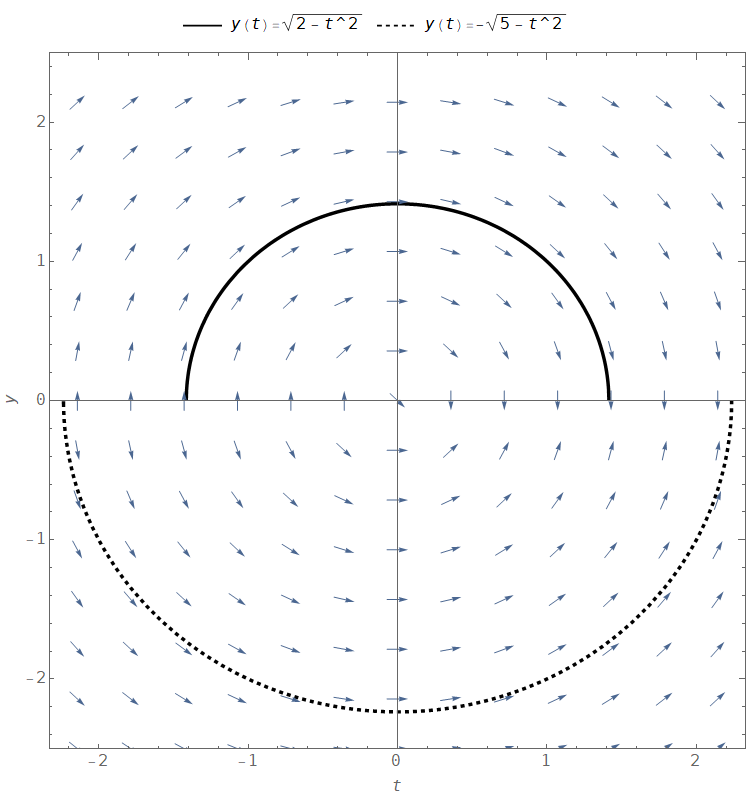
\includegraphics[width=0.4\textwidth]{exsepcircles}
	\caption{Solutions of the initial value problems given by Equation~\eqref{eq:2.2.4} and a) $y(1)=1$ and b) $y(1)=-2$, imposed on the direction field of the corresponding differential equation.}
	\label{etsepcircles}
	\end{center}
\end{figure}



\end{example}

Unfortunately, it is not always possible to extract the explicit solutions contained in an implicit one. This is illustrated in the following example. 

\begin{example}\label{example:2.2.3} 
Consider the following differential equation:
\begin{equation} \label{eq:2.2.13}
y'=\dfrac{2\,t+1}{5\,y^4+1}\,.
\end{equation}

Separating variables yields
$$
\left(5\,y^4+1\right)y'=2\,t+1\,,
$$
so that we can integrate both sides of this equation, which yields
\begin{equation} \label{eq:2.2.15}
y^5+y=t^2+t+ C\,,
\end{equation}
where $C$ is an integration constant. Clearly, this solution is an implicit one and there is no way to solve it for $y(t)$ as we did in Example~\ref{example:2.2.2}.

Suppose that we are looking for the solution satisfying the initial condition $y(2)=1$. Since both $f(t,y)$ and $f_y(t,y)$, given by
$$
-\frac{20 (2 t+1) y^3}{\left(5 y^4+1\right)^2}\,,
$$
are continuous everywhere in $\mathbb{R}^2$, Theorem~\ref{theononlineair} guarantees the existence of a unique solution of this initial value problem on some $t$- subinterval of $\left.\right]-\infty,+\infty\left[\right.$ containing $t_0=2$. Now, plugging $y(2)=1$ into Equation~\eqref{eq:2.2.15} yields $1+1=4+2+C$, so that $C=-4$. Therefore, 
$$
y^5+y=t^2+t-4
$$
is the unique solution of the initial value problem given by Equation~\eqref{eq:2.2.13} and the initial condition $y(2)=1$. Figure~\ref{etsepimplicit} shows this unique solution imposed on the direction field of Equation~\eqref{eq:2.2.13}.


\begin{figure}[H]
	\begin{center}
			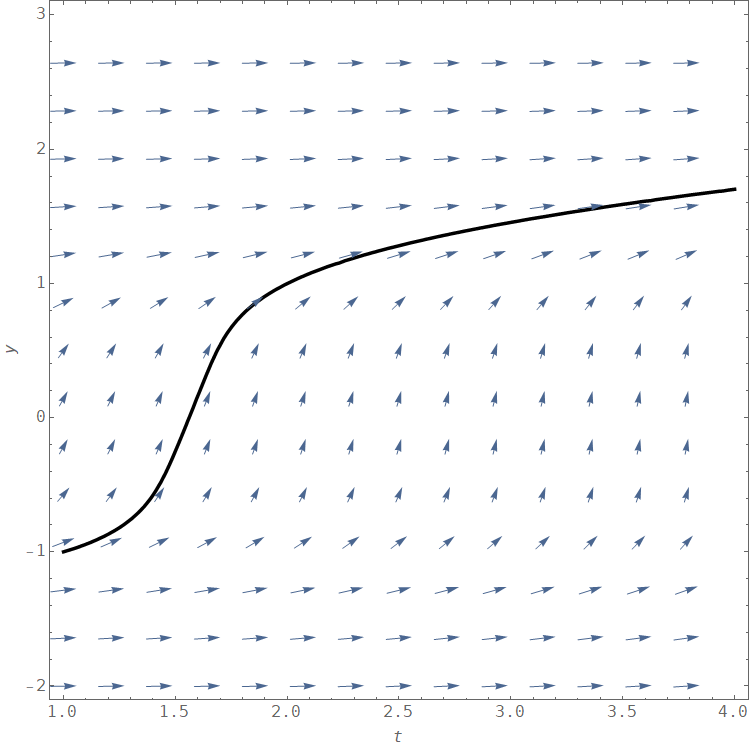
\includegraphics[width=0.4\textwidth]{exsepimplicit}
	\caption{Unique solution  of Equation~\eqref{eq:2.2.13} satisfying $y(2)=1$ imposed on the direction field of this differential equation.}
	\label{etsepimplicit}
	\end{center}
\end{figure}


\end{example}

\section{Exact differential equations}
Here, it is convenient to write first-order differential equations in the form
\begin{equation} \label{eq:2.5.1}
M(t,y)\,d t+N(t,y)\,d y=0\,.
\end{equation}
This equation  can be interpreted as
\begin{equation} \label{eq:2.5.2}
M(t,y)+N(t,y)\,\dfrac{d y}{d t}=0\,,
\end{equation}
where $t$ is the independent variable and $y$ is the dependent variable, or as
\begin{equation} \label{eq:2.5.3}
M(t,y)\,\dfrac{d t}{d y}+N(t,y)=0\,,
\end{equation}
where $y$ is the independent variable and $t$ is the dependent variable. Often the solutions of Equations~\eqref{eq:2.5.2} and \eqref{eq:2.5.3} will be implicit; that is $F(t,y)=C$. 

Since the total differential of $F(t,y)$ is given by
$$
d F=\dfrac{\partial F}{\partial t}\,d t+\dfrac{\partial F}{\partial y}\,d y\,,
$$
it immediately follows that $F(t,y)=C$ is a solution of the differential equation
\begin{equation} \label{eq:2.5.4}
F_t(t,y)\,d t+F_y(t,y)\,d y=0\,.
\end{equation}

Consequently, if we are able to find a function $F(t,y)$ for which 
\begin{equation} \label{eq:2.5.9}
F_t(t,y)=M(t,y) \mbox{\quad and \quad} F_y(t,y)=N(t,y)
\end{equation}
for  all  $(t,y)$ in some open rectangle $R$ where $F_t$ and $F_y$ are continuous, we can straightforwardly solve Equation~\eqref{eq:2.5.1}, which is then called an \textbf{exact differential equation} (\textit{exacte differentiaalvergelijking}).\index{exact differential equation}\index[aut]{exacte differentiaalvergelijking} The obvious question now of course is when a first-order differential equation is exact, i.e.\ when can we expect to find such an implicit solution $F(t,y)=C$?

Well, if there exists such a function $F(t,y)$ for which Equations~\eqref{eq:2.5.9} hold, it must also hold that 
$$
F_{ty}=F_{yt}
$$
because second-order derivatives are symmetric (Theorem of Schwarz). This implies that
\begin{equation} \label{eq:2.5.11}
F_{ty}=M_y= F_{yt}=N_t\,.
\end{equation}
So, a necessary condition for exactness is that $M_y=N_t$. This formalized in the following theorem. 


\begin{theorem}[Exactness condition]
\label{theoexact}
Suppose  $M$ and $N$ are continuous and have continuous partial derivatives
$M_y$ and $N_t$ on an open rectangle $R.$ Then
$$
M(t,y)\,d t+N(t,y)\,d y=0
$$
is exact on $R$ if and only if
\begin{equation} \label{eq:2.5.12}
M_y(t,y)=N_t(t,y)
\end{equation}
for all $(t,y)$ in $R$.
\end{theorem}


\begin{example}\label{example:2.5.3} 
Find the general solution of the following differential equation
\begin{equation} \label{eq:2.5.13}
\left(4t^3\,y^3+3\,t^2\right)\,d t+\left(3\,t^4\,y^2+6\,y^2\right)\,d y=0\,.
\end{equation}

\xhrulefill{gray}{2.5pt}Solution \xhrulefill{gray}{2.5pt}


Here we have
$$
M(t,y)=4t\,^3\,y^3+3\,t^2 \quad \text{and} \quad N(t,y)=3\,t^4\,y^2+6\,y^2\,,
$$
so we see that
$$
M_y(t,y)=N_t(t,y)=12\,t^3\,y^2
$$
for all $(t,y)$. Hence, Theorem~\ref{theoexact} implies that Equation~\eqref{eq:2.5.13} is exact from which it follows that there is a function $F$ such that
\begin{equation} \label{eq:2.5.14}
F_t(t,y)=M(t,y)=4\,t^3\,y^3+3\,t^2
\end{equation}
 and
\begin{equation} \label{eq:2.5.15}
F_y(t,y)=N(t,y)=3\,t^4\,y^2+6\,y^2
\end{equation}
 for all $(t,y)$.  To find $F$, we integrate, for instance Equation~\eqref{eq:2.5.14} with respect to $t$ to obtain
\begin{equation} \label{eq:2.5.16}
F(t,y)=t^4\,y^3+t^3+\phi(y),
\end{equation}
 where $\phi$ is a function that is independent of $t$, the variable of integration. To determine this function $\phi$ in such a way that
$F$ also satisfies Equation~\eqref{eq:2.5.15}, we assume that $\phi$ is differentiable and differentiate $F$, given by Equation~\eqref{eq:2.5.16}, with respect to $y$. This yields
$$
F_y(t,y)=3\,t^4\,y^2+\phi'(y)\,.
$$
Its right-hand side should be identical to the one of Equation~\eqref{eq:2.5.15}, so it should hold that
$$
\phi'(y)=6y^2\,.
$$
Clearly, $\phi$ can be found by integrating both sides of this equation with respect to $y$. Moreover, we may take the constant of integration to be zero because we are interested only in finding some function $F$ that satisfies Equations~\eqref{eq:2.5.14} and \eqref{eq:2.5.15}. This yields
$$
\phi (y)=2\,y^3.
$$
Finally, we substitute this expression into Equation~\eqref{eq:2.5.16} to obtain
\begin{equation} \label{eq:2.5.17}
F(t,y)=t^4\,y^3+t^3+2y^3.
\end{equation}
Consequently,
$$
t^4\,y^3+t^3+2y^3=C
$$
is the general solution of Equation~\eqref{eq:2.5.13} in an implicit form. This ultimately leads to the following explicit solution
$$
y(t)=\left(\dfrac{C-t^3}{2+t^4}\right)^{\frac{1}{3}}.
$$

The choice of first integrating Equation~\eqref{eq:2.5.14} with respect to $t$ was rather arbitrary and we may as well begin by integrating Equation~\eqref{eq:2.5.15} with respect to $y$ to obtain
\begin{equation} \label{eq:2.5.18}
F(t,y)=t^4\,y^3+2\,y^3+\psi (t)\,,
\end{equation}
 where $\psi$ is an function of $t$.  To determine it, we assume that it is differentiable and differentiate $F$ with respect to $t$,
which yields
$$
F_t(t,y)=4\,t^3\,y^3+\psi'(t)\,.
$$
 Comparing this with Equation~\eqref{eq:2.5.14} shows that the following must hold
$$
\psi'(t)=3\,t^2.
$$
Integrating this and again taking  the constant of integration to be zero yields
$$
\psi(t)=t^3.
$$
 Substituting this expression into Equation~\eqref{eq:2.5.18} yields Equation~\eqref{eq:2.5.17}. Figure~\ref{exexact} shows some solutions curves of Equation~\eqref{eq:2.5.13}, imposed on its direction field. 


\begin{figure}[H]
	\begin{center}
			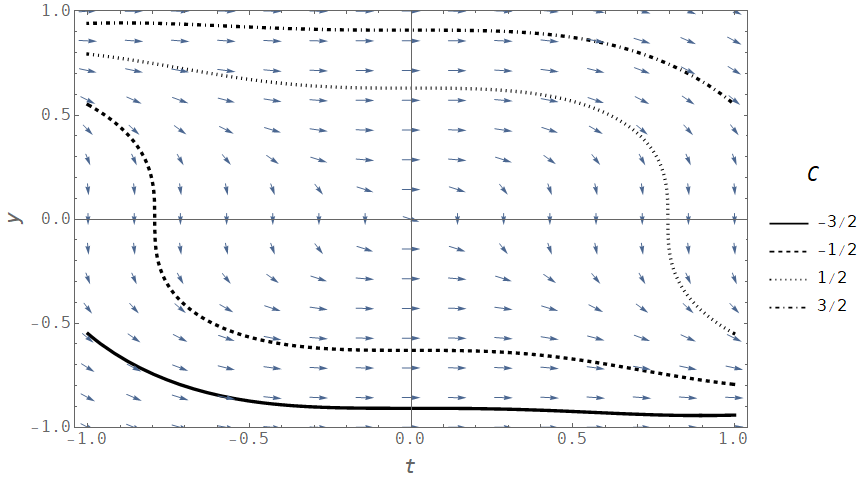
\includegraphics[width=0.6\textwidth]{exexact}
	\caption{Solution curves of Equation~\eqref{eq:2.5.13} imposed on its direction field.}
	\label{exexact}
	\end{center}
\end{figure}


\end{example}


\section{Change of variables}
There are two main reasons why we might want to consider a change of the variables in a differential equation. Firstly such a change of the dependent and/or independent variable might ease the algebraic manipulations needed to solve the differential equation analytically. In this case we typically rescale the equation's variables by means of one or more of its parameters. For instance, rescaling the dependent variable in this way, we put
$$
\tilde{y}(t)=p\,y\,,
$$
where $p$ is a arbitrary model parameter. Secondly, there are situations where a change of variables allows us to transform an non-separable to a separable equation or even a linear equation. In such cases, we will introduce
$$
y(t)=u(t)\,\phi(t)\,,
$$
where $\phi(t)$ is some known function and $u(t)$ satisfies a separable equation. 

Below we give two examples to illustrate each of these settings. 

\begin{example}
Consider the Verhulst model based on Equation~\eqref{verhulstDE} (Example~\ref{verhulstex}):
$$
P'=r\,P\left(1-\dfrac{P}{K}\right)\,.
$$

This is a separable equation, though as it involves two parameters, the algebraic manipulations might become cumbersome. Since we know from our analysis in Example~\ref{verhulstex} that the population size will always converge to $P_e=K$, it makes sense to express it relative to the carrying capacity $K$. For that reason, we put
$$
\widetilde{P}=\dfrac{P}{K}\,,
$$
so
$$
\widetilde{P}'=\dfrac{P'}{K}\,.
$$

Substituting these expressions for $P$ and $\widetilde{P}$ in  Equation~\eqref{verhulstDE} we obtain after dividing both sides by $K$
$$
\widetilde{P}'=r\,\widetilde{P}\left(1-\widetilde{P}\right)\,,
$$
which contains only one parameter, namely $r$. That parameter too can be eliminated by choosing $\tilde{t}=r\,t$ so that $d\tilde{t}=r\,d t$. In this way, we arrive at 
$$
d \widetilde{P}=\widetilde{P}\left(1-\widetilde{P}\right)d\tilde{t}\,.
$$
Separating variables yields
$$
\dfrac{d \widetilde{P}}{\widetilde{P}\left(1-\widetilde{P}\right)}=d\tilde{t}\,,
$$
whose left-hand side can be split in partial fractions:
$$
\left(\dfrac{1}{\widetilde{P}}-\dfrac{1}{\widetilde{P}-1}\right)d \widetilde{P}=d\tilde{t}\,.
$$
Integrating both sides yields
$$
\ln\left|\widetilde{P}\right|-\ln\left|\widetilde{P}-1\right|=\tilde{t}+C\,,
$$
where $C$ is an integration constant. This is the general solution of Equation~\eqref{verhulstDE}, though in implicit form. To arrive at an explicit solution, we first take the exponential of both sides:
$$
\exp\left(\ln\left|\widetilde{P}\right|-\ln\left|\widetilde{P}-1\right|\right)=e^{\tilde{t}+C}\,,
$$
which can be simplified to
$$
\dfrac{\left|\widetilde{P}\right|}{\left|\widetilde{P}-1\right|}=\widetilde{C}\,e^{\tilde t}\,,
$$
where $\widetilde{C}=e^C$, which is always greater than zero. From a biological viewpoint we know that $\widetilde{P}>0$, so $\left|\widetilde{P}\right|=\widetilde{P}$, and we can introduce
$$
\widetilde{\widetilde{C}}=\left\{\begin{array}{cl}
\widetilde{C}&\mbox{if } \widetilde{P}-1>0\,,\\
-\widetilde{C}&\mbox{if } \widetilde{P}-1<0\,,\end{array}\right.
$$
to arrive at
$$
\dfrac{\widetilde{P}}{\widetilde{P}-1}=\widetilde{\widetilde{C}}\,e^{\tilde t}\,.
$$
Solving the last equation for $\widetilde{P}$, we finally arrive at the explicit solution of Equation~\eqref{verhulstDE}:
$$
\widetilde{P}(t)=\dfrac{\widetilde{\widetilde{C}}\,e^{\tilde t}}{\widetilde{\widetilde{C}}\,e^{\tilde t}-1}\,, 
$$
or in terms of the original variables and upon dropping the tildes for the sake of readability
\begin{equation}
P(t)=K\,\dfrac{C\,e^{rt}}{C\,e^{rt}-1}\,.
\end{equation}
\end{example}

\begin{example}\label{example:2.4.1} 
Find the general solution of
\begin{equation} \label{eq:2.4.3}
y'-y=t\,y^2
\end{equation}
by introducing the change of variables $y(t)=u(t)\,e^t$.

\xhrulefill{gray}{2.5pt}Solution \xhrulefill{gray}{2.5pt}

Using the chain rule we find
$$
y'=u'\,e^t+u\,e^t\,.
$$
Substituting the expressions for $y$ and $y'$ in Equation~\eqref{eq:2.4.3}, we arrive at
$$
u'\,e^t+u\,e^t-u\,e^t=t\,u^2\,e^{2t}\,,
$$
or equivalently
$$
u'=t\,u^2\,e^t\,.
$$

Separating variables yields
$$
\dfrac{u'}{u^2}=t\,e^t\,,
$$
and integrating both sides gives
$$
-\dfrac{1}{u}=(t-1)\,e^t+C\,.
$$
Note that integration by parts was used to integrate the right-hand side.
Hence,
$$
u(t)=-\dfrac{1}{(t-1)\,e^t+C}\,,
$$
and equivalently in terms of the original variables:
$$
y(t)=-\dfrac{1}{t-1+C\,e^{-t}}.
$$
 Figure~\ref{ettrans1} shows some solutions curves of Equation~\eqref{eq:2.4.3}, imposed on its direction field. 

\begin{figure}[H]
	\begin{center}
			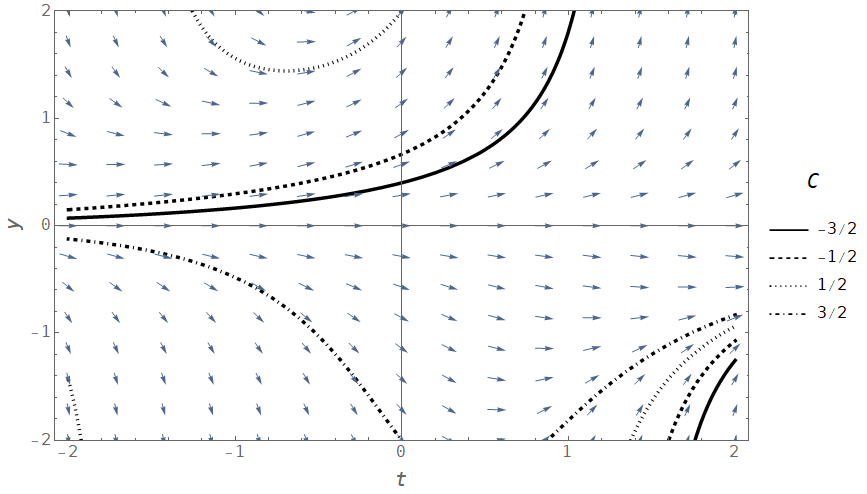
\includegraphics[width=0.6\textwidth]{extrans1}
	\caption{Solution curves of Equation~\eqref{eq:2.4.3} imposed on its direction field.}
	\label{ettrans1}
	\end{center}
\end{figure}

\end{example}

\begin{example}
First, find the general solution of 
\begin{equation} \label{eq:2.4.9}
t^2\,y'=y^2+t\,y-t^2\,.
\end{equation}
on $\left.\right]0,+\infty\left[\right.$ by introducing $y(t)=u(t)\,t$. Then, solve the initial value problem defined by this differential equation and $y(1)=2$. 

\xhrulefill{gray}{2.5pt}Solution \xhrulefill{gray}{2.5pt}

Rewriting Equation~\eqref{eq:2.4.9} in standard form and substituting both $y=u\,t$ and $y'=u'\,t+u$, we obtain
$$
u't+u =\dfrac{ (u\,t)^2+t\,(u\,t)-t^2}{t^2}
= u^2+u-1\,.
$$
So
\begin{equation} \label{eq:2.4.11}
u'\,t=u^2-1.
\end{equation}
By inspecting this equation we see that it has the constant solutions $u\equiv1$ and $u\equiv-1$. Therefore $y(t)=t$ and $y(t)=-t$ are solutions of Equation~\eqref{eq:2.4.9}. Other solutions can be found by  separating variables
$$
\dfrac{u'}{u^2-1}=\dfrac{1}{t}\,,
$$
or, after a partial fraction expansion,
$$
\dfrac{1}{2}\left[\dfrac{1}{u-1}-\dfrac{1}{u+1}\right]u'=\dfrac{1}{t}\,.
$$
 Multiplying by 2 and integrating yields
$$
\ln\left|\dfrac{u-1}{u+1}\right| =2 \ln |t|+C,
$$
 or
$$
\left|\dfrac{u-1}{u+1}\right|=e^C\,t^2\,.
$$
Consequently, we finally have
\begin{equation} \label{eq:2.4.12}
\dfrac{u-1}{u+1}=\widetilde{C}\,t^2\,.
\end{equation}
 Solving this expression for $u$ yields
$$
u(t) =\dfrac{1+\widetilde{C}\,t^2}{1-\widetilde{C}\,t^2}.
$$

Finally, we obtain that 
\begin{equation} \label{eq:2.4.13}
y(t)=u(t)\,t=t\,\dfrac{1+\widetilde{C}\,t^2}{1-\widetilde{C}\,t^2}
\end{equation}
is a solution of Equation~\eqref{eq:2.4.9} for any choice of the constant $\widetilde{C}$. Setting $\widetilde{C}=0$ in Equation~\eqref{eq:2.4.13} yields the solution $y(t)=t$. However, the other solution that we obtained by inspecting the differential equation, namely $y(t)=-t$, cannot be obtained from Equation~\eqref{eq:2.4.13}. Thus, the solutions of \eqref{eq:2.4.9} on $\left.\right]0,+\infty\left[\right.$ are $y(t)=-t$ and functions of the form given by Equation~\eqref{eq:2.4.13}.

Before trying to find the constant $\widetilde{C}$ such that Equation~\eqref{eq:2.4.13} satisfies the initial value problem, let us see what Theorem~\ref{theononlineair} tells us about the existence and uniqueness of the studied initial value problem. Writing Equation~\eqref{eq:2.4.9} in standard from we get
$$
y'=\dfrac{y^2+t\,y-t^2}{t^2}\,,
$$
from which we conclude that $f$ and $f_y$ are continuous everywhere except along the line $t=0$. In our case we have $(t_0,y_0)=(1,2)$, so we can define an open rectangle containing this point where  both $f$ and $f_y$ are continuous. Consequently, there must exist a unique solution of the considered initial value problem on some $t$-interval in $\left.\right]0,+\infty\left[\right.$ containing $t_0$. 


We could obtain $\widetilde{C}$ by imposing the initial condition $y(1)=2$ in Equation~\eqref{eq:2.4.13}, and then solve for
$\widetilde{C}$. However, it's easier to use Equation~\eqref{eq:2.4.12}. Since $u=y/t$, the initial condition $y(1)=2$ implies that $u(1)=2$.  Substituting this into Equation~\eqref{eq:2.4.12} yields $\widetilde{C}=1/3$.  Hence, the solution of the initial value problem is
$$
y=\dfrac{t\,\left(1+\frac{t^2}{3}\right)}{1-\frac{t^2}{3}}.
$$
The interval of existence of this solution is $\left]-\sqrt3,\sqrt3\right[$. However, the largest interval on which the initial value problem has a unique solution is $\left.\right]0,\sqrt3\left[\right.$. \index{interval of existence} \index[aut]{bestaansinterval}

 Figure~\ref{ettrans2} shows this unique solution imposed on its direction field. 

\begin{figure}[H]
	\begin{center}
			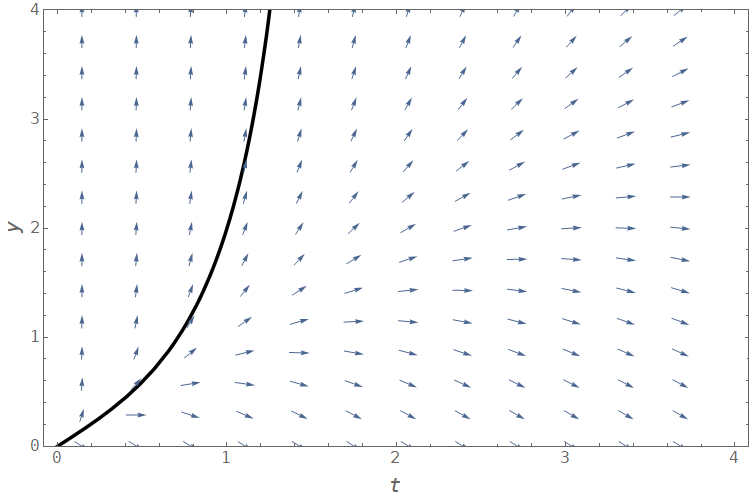
\includegraphics[width=0.6\textwidth]{extrans2}
	\caption{Unique solution of Equation~\eqref{eq:2.4.9} satisfying $y(1)=2$ imposed on its direction field.}
	\label{ettrans2}
	\end{center}
\end{figure}
\end{example}

\section{Euler's method}\label{secEuler}
\subsection{Motivation and rationale}
If the initial value problem 
\begin{equation} \label{eq:3.1.1}
y'=f(t,y),\quad y(t_0)=y_0
 \end{equation}
cannot be solved analytically,  we need numerical methods to obtain useful approximations to a solution of this initial value problem. In the remainder of this chapter, we will consider such methods. The methods that we will develop share the common feature that they lead to approximate values of the solution of the initial value problem at equally spaced points $t_0$, $t_1$, $\ldots$, $t_n$ in an interval $[t_0,t_n]$.
Hence, these points follow from
$$
t_i=t_0+i\,\Delta t,\quad i=0,1, \ldots,n\,,
$$
where
$$
\Delta t=\dfrac{t_n-t_0}{n}\,.
$$
We will denote the approximate values of the solution at these points by $y_0$, $y_1$, \ldots, $y_n$;   thus, $y_i$ is an approximation to $y(t_i)$.

The main rationale behind the  different methods that we will develop here is that the tangent line to the solution curve is known at any point $(t,y)$ in the $(t,y)$-plane, and hence this information should be somehow of use to approximate for instance $y(t_1)$, provided $y(t_0)$ is known. Essentially, we will assume that $(t_1,y_1)$  lies on a straight line passing through $(t_0,y_0)$, whose equation is given by
$$
y-y_0=m\,\left(t-t_0\right)\,,
$$
where $m$ is the line's slope whose definition depends on the method. We will first turn to the simple Euler's method. Yet, this method is so crude that it is seldom used in practice. Still, its simplicity makes it useful for illustrative purposes. Then, we will introduce the Runge-Kutta method, perhaps the most widely used method for the numerical solution of differential equations.

\subsection{The method}
\textbf{Euler's method} (\textit{methode van Euler}), illustrated in Figure~\ref{Euler}, is based on the assumption that the tangent line to the solution curve at $(t_i,y(t_i))$ approximates the solution curve itself over the interval $[t_i,t_{i+1}]$.  Since the slope of the solution curve of the differential equation
$$
y'=f(t,y)
$$
at $(t_i,y(t_i))$ is known and equals $y'(t_i)=f(t_i,y(t_i))$, the equation of the tangent line to the solution curve at $(t_i,y(t_i))$ becomes
\begin{equation} \label{eq:3.1.2}
y=y(t_i)+f(t_i,y(t_i))(t-t_i)\,.
\end{equation}


\begin{figure}
\centering
\centerline{
\subfigure[]{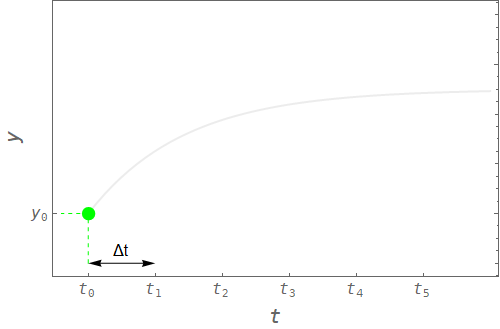
\includegraphics[width=0.45\textwidth]{Euler1}}
\hspace{1cm}
\subfigure[\label{Eulerb}]{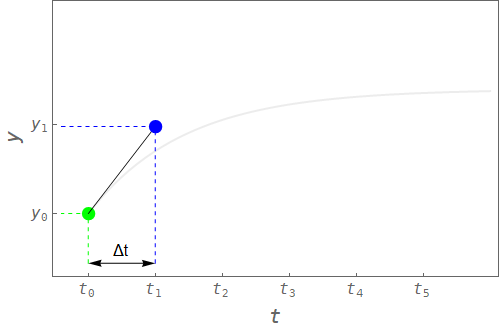
\includegraphics[width=0.45\textwidth]{Euler2}}
}
\centerline{
\subfigure[\label{Eulerc}]{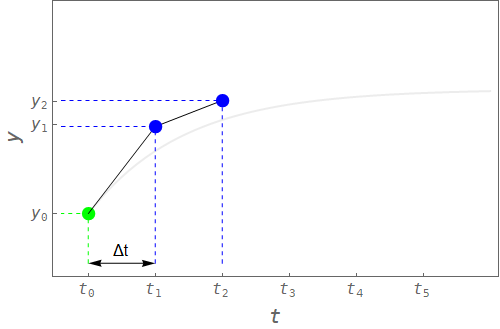
\includegraphics[width=0.45\textwidth]{Euler3}}
\hspace{1cm}
\subfigure[]{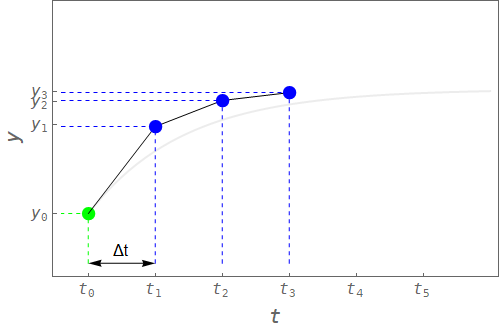
\includegraphics[width=0.45\textwidth]{Euler4}}
}
\centerline{
\subfigure[]{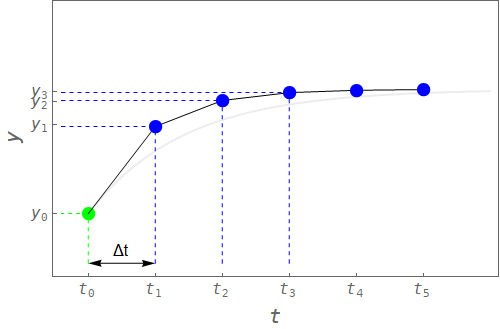
\includegraphics[width=0.45\textwidth]{Euler5}}
}
\caption{Euler's method illustrated for a generic first-order differential equation $y'=f(t,y)$: initial condition $(t_0,y_0)$ and corresponding unique solution (a), approximation of $y(t_1)$ at $t_1$ (b), approximation of $y(t_2)$ at $t_2$(c), approximation of $y(t_3)$ at $t_3$ (d) and complete numerical solution on $[t_0,t_5]$.}
\label{Euler}
\end{figure}

Suppose that $(t_i,y_i)$ is known, then Equation~\eqref{eq:3.1.2} can be used to determine $y_{i+1}$. Indeed, setting $t=t_{i+1}=t_i+\Delta t$ in Equation~\eqref{eq:3.1.2} yields
\begin{equation} \label{eq:3.1.3}
y_{i+1}=y(t_i)+\Delta t\,f(t_i,y(t_i))
\end{equation}
as an approximation to $y(t_{i+1})$. Since we are focusing on initial value problems we know that $y(t_0)=y_0$, so that we
can use Equation~\eqref{eq:3.1.3} with $i=0$ to compute
$$
y_1=y_0+\Delta t\,f(t_0,y_0)\,.
$$
This is illustrated in Figure~\ref{Eulerb}. Now, let us try find an approximation of $y(t_2)$, so we set $i=1$ in Equation~\eqref{eq:3.1.3} which yields
$$
y_2=y(t_1)+\Delta t\,f(t_1,y(t_1))\,,
$$
which we cannot evaluate since we do not know $y(t_1)$. Yet, we can replace $y(t_1)$ by its approximate value $y_1$ and redefine
$$
y_2=y_1+\Delta t\,f(t_1,y_1)\,.
$$
Having computed $y_2$, we can  compute $y_3$ in a similar fashion, i.e.
$$
y_3=y_2+\Delta t\,f(t_2,y_2)\,.
$$
In general, Euler's method starts with the known value $y(t_0)=y_0$ and computes $y_1$, $y_2$, \dots, $y_n$ successively using the following recursion equation 
\begin{equation} \label{eq:3.1.4}
y_{i+1}=y_i+\Delta t\,f(t_i,y_i)\,,
\end{equation}
for $0\le i\le n-1$.
\index{Euler's method} \index[aut]{Methode van Euler}






\subsection{Error analysis}\label{secError}

We call 
$$
e_i=y(t_i)-y_i
$$
the \textbf{error} (\textit{fout}) at the $i$-th step. Because of the initial condition $y(t_0)=y_0$, we will always have $e_0=0$.\index{error}\index[aut]{fout} However, in general
$e_i\ne0$ if $i>0$.

We encounter two sources of error in applying a numerical method to solve an initial value problem:
\begin{itemize}
\item
The formulas defining the method are based on some sort of
approximation. Errors due to the inaccuracy of the approximation are
called \textbf{truncation errors} (\textit{benaderingsfout}).\index{truncation error}\index[aut]{benaderingsfout}
\item
Computers do arithmetic with a fixed number of digits, and therefore
make errors in evaluating the formulas defining the numerical methods.
Errors due to the computer's inability to do exact arithmetic are
called \textbf{roundoff errors} (\textit{afrondingsfout}).\index{roundoff error}\index[aut]{afrondingsfout}
\end{itemize}

Since a careful analysis of roundoff error is beyond the scope of this course, we will consider only truncation errors.

There are two sources of truncation error in Euler's method:
\begin{enumerate}
\item The error committed in approximating the solution curve by the tangent line  over the interval $[t_i,t_{i+1}]$.
\item The error committed in replacing $y(t_i)$ by $y_i$ in Equation~\eqref{eq:3.1.2} and using Equation~\eqref{eq:3.1.4} rather than Equation~\eqref{eq:3.1.2} to compute $y_{i+1}$.
 \end{enumerate}

The \textbf{local truncation error} (\textit{lokale benaderingsfout})\index{local error}\index[aut]{lokale fout} at the $i$-th step $T_i$ is given by
\begin{equation} \label{eq:3.1.8}
T_i=y(t_{i+1})-y(t_i)-\Delta t\,f(t_i,y(t_i))\,.
\end{equation}
 
Since we have $t_{i+1}=t_i+\Delta t$, Taylor's theorem implies that
$$
y(t_{i+1})=y(t_i)+\Delta t\,y'(t_i)+\dfrac{\Delta t^2}{2}y''(\tilde t_i),
$$
where $\tilde t_i$ is some number between $t_i$ and $t_{i+1}$.
Since $y'(t_i)=f(t_i,y(t_i))$  this can be written as
$$
y(t_{i+1})=y(t_i)+\Delta t\,f(t_i,y(t_i))+\dfrac{\Delta t^2}{2}y''(\tilde t_i),
$$
or, equivalently,
$$
y(t_{i+1})-y(t_i)-\Delta t\,f(t_i,y(t_i))=\dfrac{\Delta t^2}{2}\,y''(\tilde t_i).
$$
Comparing this with our definition of the local truncation error (Equation~\eqref{eq:3.1.8}) shows that
$$
T_i=\dfrac{\Delta t^2}{2}\,y''(\tilde t_i).
$$
Assuming that $f$ and its partial derivatives are bounded, also its second-order derivative is bounded, so we can establish the bound
\begin{equation} \label{eq:3.1.10}
|T_i|\le\dfrac{M\,\Delta t^2}{2}\,.
\end{equation}
for $0\le i\le n-1$. The most important take-home message from this analysis is that the local truncation error of Euler's method is of \textbf{order} (\textit{orde}) $\Delta t^2$, which we sometimes write as $O\left(\Delta t^2\right)$. Note that the magnitude of the local truncation error in
Euler's method is determined by the second derivative of the solution of the initial value problem. Therefore, the local truncation error will be larger where $|y''(t)|$ is large, or smaller where $|y''(t)|$ is small.\index{order of accuracy}\index[aut]{orde van de fout}



\begin{example}
Consider once more the differential equation describing the velocity of a free-falling object (Equation~\eqref{freefall3}):
$$
m\,\dfrac{d v}{d t}=m\,g-\mu\,v\,.
$$
Let us take  $g=9.81$ \si{m.s^{-2}}, $m=75$ \si{kg}, $\mu=5.28$ \si{kg.s^{-1}}, and assume that the initial velocity of the object was 0 \si{m.s^{-1}}, so $v_0=0$ at $t = 0$ \si{s}. Figure~\ref{etEuler} shows the analytical and corresponding numerical solutions for 10, 20 and 40 steps, together with the corresponding local absolute truncation errors and a plot of the second derivative of $v(t)$. From these plots it is clear that the local absolute truncation error decreases as the number of steps increases, while there is also a clear correlation between the magnitude of the second derivative of $v(t)$ and the absolute local truncation error. 

\begin{figure}[H]
\centering
\centerline{
\subfigure[]{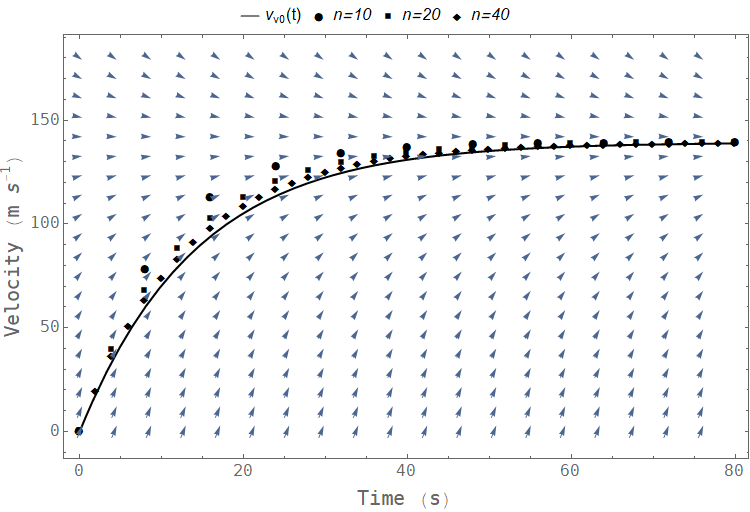
\includegraphics[width=0.45\textwidth]{exEuler1}}
\hspace{1cm}
\subfigure[]{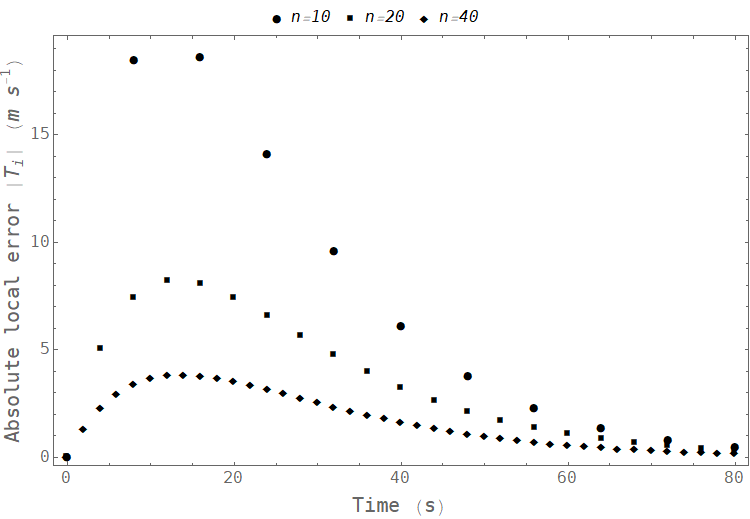
\includegraphics[width=0.45\textwidth]{exEuler1Fout}}
}
\centerline{
\subfigure[]{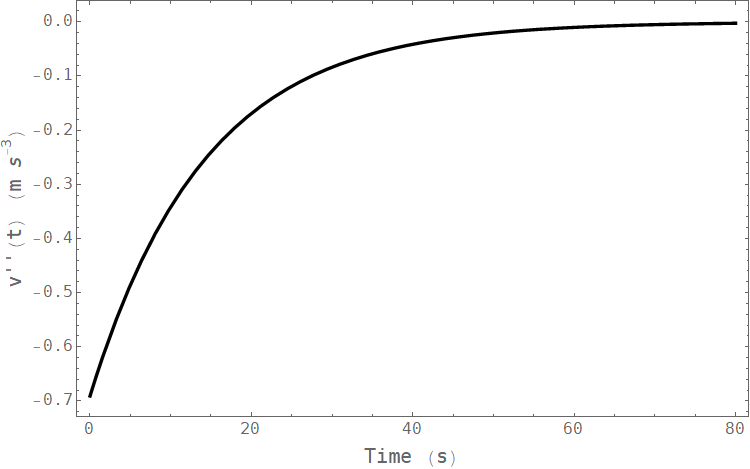
\includegraphics[width=0.45\textwidth]{exEuler1vdotdot}}
}
\caption{Analytical solution and corresponding numerical solutions of Equation~\eqref{freefall3} satisfying $v(0)=0$ obtained with Euler's method  for a different number of steps $n$ (a), together with the corresponding local truncation errors (b) and a plot of the second derivative of $v(t)$ (c).}
\label{etEuler}
\end{figure}


\end{example}

In addition to the local truncation error there also exists a \textbf{global truncation error} (\textit{globale benaderingsfout}) that is the accumulation of the local truncation errors over all iterations. A detailed analysis of the global truncation error of Euler's method is beyond the scope of this course, but it can be proofed that it is of order $\Delta t$.\index{global error}\index[aut]{globale fout}

\section{Runge-Kutta methods}\label{secRK4}
\subsection{Improving the Euler method}\label{secMidpoint}

In the previous section we saw that the global truncation error of Euler's method is $O(\Delta t)$, which would seem to imply that we can
achieve arbitrarily accurate results with Euler's method by simply choosing the step size sufficiently small. However, this
is not  a good idea, for two reasons. First, after a certain point decreasing the step size will increase roundoff errors to the point where the accuracy will deteriorate rather than improve.  The second and more important reason is that in most applications of numerical
methods the expensive part of the computation is the evaluation of the right-hand side of the differential equation. Therefore we want methods that give good results for a given number of such evaluations. 

An obvious way to improve Euler's method is by computing the slope of the line through $(t_i,y_i)$ on which we can find the approximation $y_{i+1}$ of $y(t_{i+1})$ in a more meaningful way. In Euler's method this slope is completely determined by the slope of the tangent to the solution curve passing through $(t_i,y_i)$. Yet, if $f(t,y)$ changes rapidly as $t$ increases, this slope will change rapidly as we move away from $(t_i,y_i)$, so it might make sense to determine the slope of the approximating line on the basis of two or more points near $(t_i,y_i)$. 

The improved Euler method, the \textbf{Midpoint method} (\textit{Midpointmethode}) does this by considering a line through $(t_i,y(t_i))$ with
slope
$$
m_i=\dfrac{f(t_i,y(t_i))+f(t_{i+1},y(t_{i+1}))}{2}\;
$$
that is, $m_i$ is the average of the slopes of the tangent lines to the solution curve at the endpoints of $[t_i,t_{i+1}]$. The equation of the approximating line therefore becomes
\begin{equation} \label{eq:3.2.2}
y=y(t_i)+\dfrac{f(t_i,y(t_i))+f(t_{i+1},y(t_{i+1}))}{2}(t-t_i).
\end{equation}
Setting $t=t_{i+1}=t_i+\Delta t$ in Equation \eqref{eq:3.2.2} yields
\begin{equation} \label{eq:3.2.3}
y_{i+1}=y(t_i)+\dfrac{\Delta t}{2}\left(f(t_i,y(t_i))+f(t_{i+1},y(t_{i+1}))\right)
\end{equation}
as an approximation to $y(t_{i+1})$. As in our derivation of Euler's method, we have to replace $y(t_i)$ in this equation by its
approximate value $y_i$ because the former is unknown if $i>0$. In this way, Equation~\eqref{eq:3.2.3} becomes
$$
y_{i+1}=y_i+\dfrac{\Delta t}{2}\left(f(t_i,y_i)+f(t_{i+1},y(t_{i+1})\right)\,.
$$
However, this still will not work, because we do not know $y(t_{i+1})$, which appears in the right-hand side of this equation. We overcome this by replacing $y(t_{i+1})$ by $y_i+\Delta t\,f(t_i,y_i)$, the value that the  Euler method would assign to $y_{i+1}$ when applied to the point $(t_i,y_i)$. Thus,  the improved Euler method starts with the known value $y(t_0)=y_0$ and computes $y_1$, $y_2$, \dots, $y_n$ successively with the following recursive equation:
\begin{equation} \label{eq:3.2.4}
y_{i+1}=y_i+\dfrac{\Delta t}{2}\left(f(t_i,y_i)+f(t_{i+1},y_i+\Delta t\,f(t_i,y_i))\right).
\end{equation}
The computation indicated here can be conveniently organized as follows: given $y_i$, compute
\begin{eqnarray*}
m_{1i}&=&f(t_i,y_i),\\
m_{2i}&=&f\left(t_i+\Delta t,y_i+\Delta t\,m_{1i}\right).\\
\end{eqnarray*}

Equation \eqref{eq:3.2.4} can be rewritten as

\begin{equation} \label{eq:3.3.4}
y_{i+1}=y_i+\dfrac{\Delta t}{2}(m_{1i}+m_{2i})
\end{equation}

The improved Euler method requires two evaluations of $f(t,y)$ per step, while Euler's method requires only one.  However,  the local truncation error with the improved Euler method is $O\left(\Delta t^3\right)$, rather than $O\left(\Delta t^2\right)$ as with Euler's method. Therefore the global truncation error with the improved Euler method is $O\left(\Delta t^2\right)$, which makes this a second-order method.

We note that the magnitude of the local truncation error in the improved Euler method  is determined by the third derivative of the solution of the initial value problem. Therefore the local truncation error will be larger where $|y'''(t)|$ is large, or smaller where $|y'''(t)|$ is small.

\subsection{The methods of Runge and Kutta}\label{secRK}
One of the most widely used methods for solving differential equations numerically is the so-called \textbf{Runge-Kutta method} (\textit{Runge-Kutta methode}). For this method it can be shown that the magnitude of the local truncation error is determined by the fifth derivative of the solution of the initial value problem. Therefore the local truncation error will be larger where $|y^{(5)}(t)|$ is large, or smaller where $|y^{(5)}(t)|$ is small. The Runge-Kutta method is sufficiently accurate for most applications.

The Runge-Kutta method computes approximate values $y_1$, $y_2$, \dots, $y_n$ of the solution of the initial value problem given by Equation~\eqref{eq:3.1.1} at $t_0$, $t_0+\Delta t$, \dots, $t_0+n\,\Delta t$ as follows. First, given $y_i$, compute the slope of the tangent line to the solution curve at four points, i.e.
\begin{eqnarray*} 
m_{1i}&=&f(t_i,y_i),\\
m_{2i}&=&f\left(t_i+\dfrac{\Delta t}{2},y_i+\dfrac{\Delta t}{2}m_{1i}\right),\\
m_{3i}&=&f\left(t_i+\dfrac{\Delta t}{2},y_i+\dfrac{\Delta t}{2}m_{2i}\right),\\
m_{4i}&=&f(t_i+\Delta t,y_i+\Delta t m_{3i})\,.
\end{eqnarray*}
Finally, compute $y_{i+1}$ on the basis of a weighted average of these four slopes: 
\begin{equation} \label{eq:3.4.4}
y_{i+1}=y_i+\dfrac{\Delta t}{6}\left(m_{1i}+2\,m_{2i}+2\,m_{3i}+m_{4i}\right).
\end{equation}


\begin{example}
For what concerns Equation~\eqref{freefall3}, Figure~\ref{etRK4} shows its analytical solution and corresponding numerical solutions for 10, 20 and 40 steps if $v_0=0$, together with the corresponding local absolute truncation errors. From these plots it is again clear that the local absolute truncation error decreases as the number of steps increases. Comparing this figure with the one obtained when using Euler's method, it is obvious that the Runge-Kutta method is much more accurate because the magnitude of the local truncation is always much lower than in the case of Euler's method, irrespective of the number of steps and time. 

\begin{figure}[H]
\centering
\centerline{
\subfigure[]{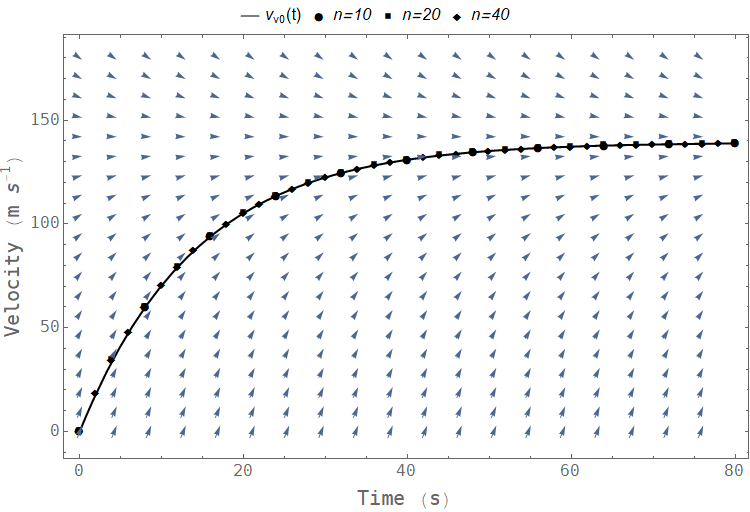
\includegraphics[width=0.45\textwidth]{exRK4}}
\hspace{1cm}
\subfigure[]{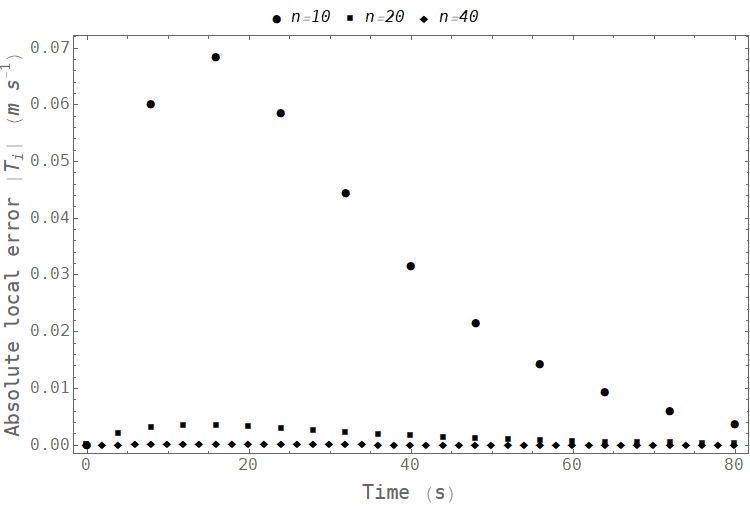
\includegraphics[width=0.45\textwidth]{exRK4Fout}}
}
\caption{Analytical solution and corresponding numerical solutions of Equation~\eqref{freefall3} satisfying $v(0)=0$ obtained with the Runge-Kutta method for a different number of steps $n$ (a), together with the corresponding local truncation errors (b).}
\label{etRK4}
\end{figure}

\end{example}

\newpage
\section{Exercises}
\renewcommand{\ExerciseListName}{Assignement}

%\subsection{Analytische methoden}
\begin{Exercise}Solve the following differential equations by separating the variables. Determine the largest possible solution interval in each case. \par
\begin{multicols}{2}
    \Question $-t^2 \, dy = \left( y + 3 \right) \, dt$
    %\item $y' = \dfrac{2 t - 1}{2 y - 5}$
    \Question $y' = 1 + y^2$
    %\item $y' = y \csc t$
    \Question $t^3 \, dy + y^3 \, dt = 0$
    %\item $my - n t y' = 0$
    \Question $e^t y' = e^y$
    %\item $y' = \sqrt{a^2 - y^2}$
    \Question $t^2 y y' = e^y$
    \EndCurrentQuestion
\end{multicols}
\end{Exercise}

\setboolean{firstanswerofthechapter}{true} To determine the largest possible solution interval, we distinguish between linear and nonlinear first order differential equations. In the case of a linear first order differential equation, we put the differential equation in the form $y' + p(t)y = q(t)$ and examine the continuity of $p(t)$ and $q(t)$. For a nonlinear differential equation, we put it in the form $y' = f(t, y)$ and examine both the continuity of $f(t,y)$ and $\dfrac{\partial f(t,y)}{\partial y}$.

\begin{Answer}\phantom{}    
        \Question $y(t) = - 3 + C\,e^{\frac{1}{t}}$, \quad solution intervals: $t \in ]-\infty,0[$ of $t \in ]0,+\infty[$
        \Question $y(t) = \tan(t+C)$, \quad solution interval: $t \in ]-\infty,+\infty[$ en $y\in ]-\infty,+\infty[$
        \Question $y(t) = \pm \dfrac{t}{\sqrt{Ct^2-1}}$,\quad solution intervals: $t \in ]-\infty,0[$ of $t \in ]0, +\infty[$ en $y \in ]-\infty, +\infty[$ %$t \in \left]-\infty,-\dfrac{1}{\sqrt{C}}\right[$ of $t \in \left]\dfrac{1}{\sqrt{C}},+\infty\right[$
        \Question $y(t) = -\ln{\Big|e^{-t} - C\Big|}$,\quad solution interval: $t \in ]-\infty,+\infty[$ en $y \in ]-\infty,+\infty[$
        \Question $\dfrac{1+y}{e^y}=\dfrac{1}{t}+C$,\quad solution intervals: $t \in ]-\infty,0[$ of $t \in ]0,+\infty[$ en $y \in ]-\infty,0[$ of $y \in ]0,+\infty[$
\end{Answer}
\setboolean{firstanswerofthechapter}{false}

\begin{Exercise}Solve the following exact differential equations.
    \begin{multicols}{2}
    \Question $\left( 2 t y + 3 t^2 y^2 \right) \, dt + \left( t^2 + 2 t^3 y \right) \, dy = 0 $
    \Question $\left( t + 3 y \right)\, d t + 3 \left( t - y \right)\, d y = 0$
    \Question $ y' \left( t - \sin(y) \right) + y = 0 $
    %\item $\dfrac{y\; d t - t\; d y}{t^2 + y^2} = 0 $
    %\item $\left( \dfrac{1}{y} - \dfrac{y}{t^2} \right) d t + \left( \dfrac{1}{t} - \dfrac{t}{y^2} \right) d y  = 0$
    \Question $\left( 1 + y\, e^{ty} \right) \, dt + \left( 1 + t\, e^{ty} \right)\, dy = 0$
    %\item $\dfrac{t y\; d t - t^2\; d y}{y^2 \sqrt{t^2 + y^2}} = 0 $
    %\item $\left [ 1 - \dfrac{4 y^2}{\left( t - y \right)^2} \right ] d t = \left [ 1 - \dfrac{4 t^2}{\left( t - y \right)^2} \right ] d y $
    %\item $\left(\sin t + \ln |y| \right) d t + \left( \dfrac{t}{y} + e^{2y}\right)d y = 0$
    \EndCurrentQuestion
    \end{multicols}
\end{Exercise}

\begin{Answer}
    \begin{multicols}{2}
    \Question $t^2y+t^3y^2 = C$ %$y = \dfrac{-t\pm \sqrt{t^2+Ct}}{2t^2}$
    \Question $\dfrac{t^2}{2} +3yt-3\dfrac{y^2}{2} = C$ %$y = t\pm \dfrac{\sqrt{12C^2t^2+3}}{3C}$
    \Question $ty + \cos (y) = C$
    \Question $t+y+e^{ty}=C$
    \EndCurrentQuestion
    \end{multicols}
\end{Answer}

%\item Is volgende vergelijking exact? Bepaal indien mogelijk de oplossing van dit beginwaardeprobleem.
%  \begin{equation*} \label{eq:koenie2}
%  y^2\,d\,t+(2\,t\,y+1)\,{\rm d}y=0,~~y(0)=1\,.
%  \end{equation*}

\begin{Exercise}Consider the differential equation
\[ 2y^{a-1}\left(1+\sin(2t)\right)y' + 3t^2+y^a\cos(2t)=0.\]
	\Question For which values of $a$ is the differential equation exact?
	\Question Determine the general solution of this differential equation for the value of $a$ found in a).
\end{Exercise}

\begin{Answer}
    \begin{multicols}{2}
        \Question $a = 4$
        \Question $y(t) = \Bigg(\dfrac{2\left(C - t^3\right)}{1 + \sin(2t)}\Bigg)^{1/4}$
    \EndCurrentQuestion
    \end{multicols}
\end{Answer}

\begin{Exercise} Consider the differential equation
\begin{equation*}\label{eqk1}
\frac{y'}{y}=\frac{e^{2a}+\sin(t)+1}{\cos(t) -2\,e^a\,t-a}\,.
\end{equation*}
\Question For what value of $a$ is the differential equation exact? 
\Question Then determine the unique solution corresponding to initial value $y(0)=-1$.
\Question What is the largest open rectangle in the $(t,y)$-plane within which the conditions of Theorem 3.3 are satisfied?
\end{Exercise}

\begin{Answer}
        \Question $a = 0$
        \Question $y(t) = \dfrac{1}{-\cos (t) + 2t}$
        \Question $]-\infty, 0.450184[ \times ]-\infty,+\infty[$ with $0.450184$ the solution of $\cos(t)=2t$ (determined in Mathematica).
    \EndCurrentQuestion
\end{Answer}

\begin{Exercise} Solve the linear differential equations below.
\begin{multicols}{2}

%\begin{multicols}{2}
\Question $y' + 2 y = 3 t + 1$
%\item $y'-3y=e^{3t}(t+2)+e^{-t}$
%\item $y'+4y=e^{4t}(2t^2-5t+1)$
%\item $y'+3y=\sin 2t$

%\item $y'+2y=3e^{-5t}\cos t$
%\item $y'-3y=t^2e^{3t}\sin t$
%\item $y' + \dfrac{t y}{1 + t^2} = \dfrac{1}{1 + t^2}$

%\item $y' + \dfrac{y}{t - 1} = \dfrac{6 t^2 + t + 5}{t - 1}$
%\item $\left( t^2 + 1 \right) y' - t y = 4 \left( t^2 + 1 \right)$
%\item $y' + y \sin  t = \sin   2t$
\Question $\left( 1 - t^2 \right) y' + t y = t^3 \qquad\left(t \in \, ] -1 , 1 [\right)$
%\item $\left( t + 3 \right) y' - 2 y = \left( t + 3 \right)^3\; \sqrt{t + 3}$
%\item $t  y' \ln  t + y = t^2 \ln t$

\Question $t y' - y = \left( t - 1 \right) e^t$
%\item $dr + \left( 2 r \cot \theta + \cos \theta \right) d\theta = 0$
%\item $y' + \dfrac{y}{\sqrt{t^2 + 1}} = t - \sqrt{t^2 + 1}$
\Question $y' \sqrt{1 - t^2} + y = 1$
%\item $\left( 1 + \sin  y \right) d t = \left( \cos  y - t \sec y - t \tan y \right) d y$ %\hfill  \left(\mbox{werk met } \dfrac{d t}{d y}\right)$

%\item $y' + \dfrac{2}{t}y = -t\qquad\mbox{met}\quad y(1)=\dfrac{3}{4}$
%\end{multicols}
\EndCurrentQuestion
\end{multicols}
\end{Exercise}

\begin{Answer}
    \begin{multicols}{2}
        \Question $y(t) = -\dfrac{1}{4} + \dfrac{3t}{2} + Ce^{-2t}$
        \Question $y(t) = 2 - t^2 + C\sqrt{1-t^2}$
        \Question $y(t) = C|t| - e^{t}$
        \Question $y(t) = 1 + Ce^{-\arcsin(t)}$
        \EndCurrentQuestion
    \end{multicols}
\end{Answer}

\begin{Exercise} Determine the general solution of the differential equations below.
\begin{multicols}{2}

    \Question $\left( 1 + t \right) y \, d t + ( 1 - y ) t\, d y = 0$
    \Question $(t+\sin (y))\,d t+(t\cos (y) -2\,y)\,dy=0$
    \Question $\left( 1 + e^{3t} \right) \, d y + 3 y e^{3t}\, d t = 0$
    \Question $y'-y=2(t-1)\cos (t)$
%\item $\left( t \ln  y - y \sin  t \right) d t + \left( \ln  y + \cos  t + \dfrac{t^2}{2 y} \right) d y = 0 $
\Question $y' - t y = t^3$
    \Question $y\,y'=t^2+2$
    \Question $\left(y^2-1\right) y'=2$
%\item $y' + y\, \tanh (t) = e^{2t}$

%\item $\left( t^3 + t^2 + t + 1 \right) y' = \left( 3 t^2 + 2 t + 1 \right) y $
\Question $( 2 y + 3 ) \, d t = ( t + 1 ) \, d y$
\Question $2 t y \, d t + \left( 3 t^2 + 1 \right) \, d y = 0$
%\item $t y' + y = t^2 \cos t$
\Question $\left( y - \dfrac{1}{1 + t^2} \right) \, d t + t \, d y = 0 $
%\item $t^2 y' + 2ty - 1 =0$
\Question $\sin  (t)  \cos  (t) \, d y = \left( \sin  (t) + y \cos ^2 (t) \right) \, d t$
%\item $\, dr + r \tan \theta \; \theta = 0 $
%\item $\left( t - y^2 t \right) d t + \left( y - t^2 y \right) d y = 0$
%\item $tyy' = 1 + t^2 + y^2 + t^2y^2$
\Question $\left(1 + e^{-t}\right) y' \sin (y) + \cos (y) = 0$
%\item $y'+\dfrac{y}{t^2} = e^\frac{1}{t}\qquad\mbox{met}\quad y(1)=3e$
\Question $\left( y - \cos  (t) \right) \, d t + \left( t + 1 \right) \, d y = 0$
%\item $y' - \dfrac{y}{t} = y \ln t \qquad\mbox{met}\quad y(1)=1$
\EndCurrentQuestion
    
\end{multicols}
\end{Exercise}

\begin{Answer}\phantom{}
    \begin{multicols}{2}
        \Question $\ln|y(t)|- y = -\ln|t| - t + C$ %$y(t) = - ProductLog\Big[ -\dfrac{e^{-t-C_1}}{t} \Big]$
        \Question $t \sin(y(t)) - y(t)^2 + \dfrac{t^2}{2} = C$
        \Question $y(t) = \dfrac{C}{1 + e^{3t}}$
        \Question $y(t) = Ce^{t} + \cos(t) - t\cos(t) + t\sin(t)$
        \Question $y(t) = Ce^{\frac{t^2}{2}} - 2 - t^2$
        \Question $y(t) = \pm \sqrt{\dfrac{2}{3}t^3 + 4t + C}$
        \Question $y(t)^3-3y(t) = 6t + C$
        \Question $y(t) = -\dfrac{3}{2} + C(1+t)^2$
        \Question $y(t) = \dfrac{C}{|1+3t^2|^{1/3}}$
        \Question $y(t) = \dfrac{\arctan(t)}{t} +  \dfrac{C}{t}$
        \Question $y(t) = C|\sin(t)| + \sin(t)\Big( \ln\big|\sin(t)\big| - \ln\big|\cos(t)\big| \big)$
        \Question $y(t) = \arccos\Big( C\left(1+e^{t}\right) \Big)$
        \Question $y(t) = \dfrac{C+\sin(t)}{1+t}$
        \EndCurrentQuestion
    \end{multicols}
\end{Answer}

%\item Bepaal de unieke oplossing van de onderstaande beginwaardeproblemen.
%\begin{enumerate}
%\item $t\,y'+y=t^2\,\cos t,\qquad \mbox{met}\quad y(\pi)=\dfrac{\sqrt3}{\pi}-2\quad\mbox{en}\quad t,y\in\mathbb{R}_0$
%\item $y'+\,y\,\sin t=\sin (2\,t),\qquad \mbox{met}\quad y\,\left(\dfrac{\pi}{2}\right)=\sqrt 5+2$
%\item $y'=-\dfrac{t\cos t}{1-6\,y^5},\qquad \mbox{met}\quad y(\pi)=0$
%\end{enumerate}


\begin{Exercise}  Consider the differential equation
$$y'+\left(\cot(t)\right)y=2\,\cos (t)\,.$$

\Question Determine the intervals over which Theorem 3.1 guarantees a unique solution.
\Question Determine the unique solution of the differential equation if $y(\pi/2)=2$. Also, point out in which interval this is guaranteed to be the unique solution of the initial value problem by Theorem 3.1.
\end{Exercise}

\begin{Answer}\phantom{}
        \Question Solution intervals: $\mathbb{R}\setminus\{k\pi,k\in \mathbb{Z}\}$
        \Question $y(t) = \sin (t) + \dfrac{1}{\sin (t)}$ %$y(t) = -\dfrac{1}{2}\big( \cos(2t) - 3 \big)\csc(t)$
\end{Answer}

\begin{Exercise} Consider the differential equation 
$$
y'+\left(\tan (t)\right)\,y=\cos^2 (t)\,,\quad y(0)=-1\,.
$$
\Question Determine the largest $t$-interval over which Theorem 3.1 guarantees the existence of a unique solution.
\Question Solve the initial value problem.
\Question Determine the equilibrium points of the differential equation and their stability.
\end{Exercise}


\begin{Answer}\phantom{}
         \Question solution interval: $t \in \left]-\dfrac{\pi}{2},\dfrac{\pi}{2}\right[$
        \Question $y(t) = \cos(t)\big(\sin(t) - 1 \big)$
        \Question $y' = 0 \Leftrightarrow y_e = \dfrac{\cos^3(t)}{\sin(t)}$. This is not a constant value for $y_e$. There are no equilibrium points. %De evenwichtspunten worden gegeven door $y_e(t) = \dfrac{\cos^3(t)}{\sin(t)}$. Als $t = \pi/2$ is $y_(t = \pi/2) = 0$. Dit evenwichtspunt blijkt OS te zijn.
\end{Answer}

%\item Bepaal de unieke oplossing van het beginwaardeprobleem
%$$
%\sqrt{y}\,\left(3\,y'+y\right)=t\,,\qquad y(0)=1\,.
%$$
%Bepaal vervolgens de evenwichtspunten van de bovenstaande differentiaalvergelijking.


%\item Bepaal de algemene oplossing en de evenwichtspunten van:
%    $$t'=t^2-2\,t+2\,.$$



\begin{Exercise} Determine the unique solution of the initial value problem
\begin{equation*}
y'=\left\{\setlength{\arraycolsep}{2pt} \begin{array}{lcl} 
\cos^2 (t), & & \quad \text{ if }  t>2,\\[0.4cm]
\dfrac{y^2}{3}, & & \hspace{0.5cm} \text{else}, 
\end{array}\right.
\end{equation*}
where $y(0)=1$.
\end{Exercise}

\begin{Answer} First, we solve the differential equation $y' = \dfrac{y^2}{3}$ for $t \leq 2$ with $y(0) = 1$. We arrive at the exact solution $y(t) = \dfrac{3}{3-t}$ if $t \leq 2$. If we use $t = 2$, then we get $y(2) = 3$. We now use this as the initial condition for the differential equation $y'(t) = \cos^2(t)$. We arrive at the exact solution $y(t) = \dfrac{1}{4}\Big( 8 + 2t - \sin(4) + \sin(2t) \Big)$ if $t > 2$.\\

Concluded:
\begin{equation*}
y(t)=\left\{\setlength{\arraycolsep}{2pt} \begin{array}{ll} 
\dfrac{3}{3-t}, & \quad\text{if }t \leq 2,\\[0.4cm]
\dfrac{1}{4}\Big( 8 + 2t - \sin(4) + \sin(2t) \Big), & \quad\text{als }t > 2.
\end{array}\right.
\end{equation*}
\end{Answer}

%%%%%%%%%%%%%%%%%%%%%%%%%%%%%%
%Geschrapt
\iffalse
\item Solve the differential equations below by using the given substitution.
\begin{enumerate}
%\begin{multicols}{2}
%\item $y \left( ty - 1 \right) d t + t \left( t^2 y^2 - 2 t y + 3 \right) d y = 0$   TE MOEILIJK
\item $y \left( 1 + 2 t y \right)\, d t + t \left( 1 - ty \right) \, d y = 0$\hfill $u = ty$
%\item $t^2 y^3\; d t  + t^4 y^3\; d y = 0$   GEEN SUBS NODIG
\item $t^2 \cos  (y)\; y' = 2 t \sin  (y) - 1$\hfill $u=\sin (y)$
%\item $y' + 2 t ( y - t ) = t^3 ( y - t )^2 + 1$   GEEN MOOIE UITKOMST
\item $y y' + \left( y^2 - 1 \right) t = t^3$\hfill $u=\dfrac{y^2-1}{2}$

\item $y' + t y = t^3 y^3$ \hfill $u=y^{-2}$
%\item $\left( t + y \right) d t = \left( t - y \right) d y$
\item $\left( 1 - t^2 \right) y' - t y = a t y^2$\hfill $u=\dfrac{1}{y}$
\item $3 y' + y = \left( 1 - t \right) y^4$\hfill $u=y^{-3}$
\item $\left( t^2 + y^2 \right) \, d t = t y\, d y $\hfill $u=\dfrac{y}{t}$
%\item $y' = \dfrac{t - y}{t}$
%\item $t^3  y^2 + 2 t y = y'$
%\item $t^2 y\; d t = \left( t^3 + y^3 \right) d y$
%\item $y' + y + \left(\sin t - \cos t\right) y^2=0$\hfill $u=\dfrac{1}{y}$
%\item $ty' = y + y^2$
%\item $y'-\dfrac{t^2y}{2} = y^3t^2e^{-t^3}$
%\item $\left( 2 t + y\right) d t + \left( t + 2 y \right) d y = 0$
%\item $\left( 7 t + 9 y \right) y' + 4 t + 6 y = 0 $
%\item $\left( 2 y + \sqrt{2 t^2 + y^2}\right) d t = 2 t\; d y$
%\item $y' = \dfrac{t}{y} e^{-\frac{y}{t}} + \dfrac{y}{t}$
%\item $t \cos \dfrac{y}{t} \; y' = y \cos \dfrac{y}{t} - t$\hfill $u=\dfrac{y}{t}$

\item $ty' + y = t^3y^{-2}$\hfill $u=y^3$
%\item $y' - \dfrac{y}{t} = ay\ln t$\hfill $u=\dfrac{y}{t}$
\item $y'  = \left( y - t \right)^2$\hfill $u=y-t$
%\item $y' = \sinh^2 \left( t + y \right)$
%\item $d y = \left( 3 t + y \right) d t$
%\item $\left( t + y - 3 \right) d y = 2 \left( t + y \right) d t$
\item $e^y y' = 2 \left( t + e^y \right) - 1$\hfill $u=e^y$
%\item $\left( y \cos (ty) - \sin  (ty) \right) d t + t \cos (ty) d y = 0 $ \hfill $u=ty$
%\item $2 y y' \left( t - y^2 \right) = t + y^2$
%\item $2 t y y' + \left( t - 1 \right)\; y^2 = t^2 e^t \hspace{1cm} \left( tz = y^2 \right)$
%\end{multicols}
\end{enumerate}
\fi
%%%%%%%%%%%%%%%%%%%%%%%%%%%%%%

%\item Los op:
%\begin{enumerate}
%\item $t^2\,y\,y'=e^y,\qquad y(1)=0$

%\item $(t-y^2\,t)+(y-t^2\,y)\,y'=0,~~y(0)=0$

%\item De desintegratiesnelheid $d\,N/d\,t$ van een radioactieve stof is recht evenredig met $N$, het aantal nog voorhanden zijnde deeltjes. In 1600 jaar wordt door straling de helft van de oorspronkelijke aanwezige hoeveelheid omgezet. Hoelang duurt het eer $5\%$ ervan is omgezet?

%\item $(t-\sin y)\,y'+y=0,~~y(0)=\dfrac{\pi}{4}$
%\end{enumerate}

\begin{Exercise}
    \Question Solve Equation (\ref{eentank}) (mass balance).
\end{Exercise}

\begin{Answer}
\Question $C(t) = \dfrac{qC_{in}}{q + rV}+ C e^{-t(r+\frac{q}{V})}$
\end{Answer}


\begin{Exercise}
    \Question In a chemical reaction, one molecule of substance $P$ and one molecule of substance $Q$ together form one molecule of the substance $R$.
    There are $p$ [--] molecules $P$ and $q$ [--] molecules $Q$ present at the start of the reaction. The number of molecules $R$ at time $t$ [T] is $x$. The rate at which $R$ is formed at any time during the reaction is directly proportional to the product of the remaining numbers of molecules $P$ and $Q$:
    \[ \dfrac{d x}{d t} = k ( p - x ) ( q - x ),\]
    met $k >0$. Determine $x$ with respect to $t$ if $x = 0$ for $t = 0$.
\end{Exercise}

\begin{Answer}
    \Question $C(t) = \dfrac{qC_{in}}{q + rV}+ C e^{-t(r+\frac{q}{V})}$
\end{Answer}

\begin{Exercise}
    \Question The disintegration rate $\dfrac{d N}{d t}$ [$T^{-1}$] of a radioactive substance is directly proportional to $N$ [--], the number of particles. In 1600 years, radiation converts half of what was originally present into
    converted. How long does it take to convert $5 \%$ of it?
\end{Exercise}

\begin{Answer}
    \Question The differential equation is $N' = -\lambda N$ with $N(0) = N_0$. The general solution is $N(t) = N_0e^{-\lambda t}$. If $t = 1600$ is $N(1600) = N_0/2$. From this it follows that $\lambda = \dfrac{\ln(1/2)}{-1600}$ or approximately $0.0004332$. \\
    To calculate how long it takes for 5\% to convert, we need to solve the equation\\
    $N(t_5) = N_0e^{-\lambda t_5} = 0.95N_0$. We get:
    \[t_5 = \dfrac{\ln(0.95)}{- 0.0004332} \approx 118.37 \mbox{ years}. \]
\end{Answer}

\begin{Exercise}
    \Question A rocket with mass $M$ (fuel included) is shot up vertically and undergoes frictional resistance directly proportional to the speed $v$ achieved. Per unit of time, fuel with mass $m$ is consumed. The products of combustion are emitted at a constant velocity $- v_0$ with respect to the rocket. The differential equation describing the change in velocity is given by:
    \[ \dfrac{d v}{d t} + \dfrac{K}{M - m t} v = - g + \dfrac{m v_0}{M - m t} \qquad (K \mbox{ is constant}).\]
    Determine the function that expresses $v$ as a function of $t$ if the rocket departs from rest.
\end{Exercise}

\begin{Answer}
    \Question $v(t) = \dfrac{g(M-mt)}{m-K} + \dfrac{m v_0}{K} - \dfrac{m v_0M^{\frac{-K}{m}}}{K}(M-mt)^{\frac{K}{m}}-\dfrac{gM^{1-\frac{K}{m}}}{m-K}(M-mt)^{\frac{K}{m}}$ %$v(t) = \dfrac{1}{K(K-m)}(-M)^{-K/m}\Bigg( gK\Big( (-M)^{1+K/m} + m (-M)^{K/m}t + M(-M + mt)^{K/m} \Big) + v0(K - m)m\Big( (-M)^{K/m} - (-M + mt)^{K/m} \Big) \Bigg)$
\end{Answer}
%%%%%%%%%%%%%%%%%%%%%%%%
%oude oefeningen, nederlands zonder oefeningenomgeving
%%%%%%%%%%%%%%%%%%%%%%%%

% \newpage
% \section{Exercises}


% %\subsection{Analytical methods}
% \begin{enumerate}
% \item Solve the following differential equations by separation of variables. Determine the largest possible solution interval in each case.\par
% \begin{multicols}{2}


% \begin{enumerate}
% \item $-t^2 \, dy = \left( y + 3 \right) \, dt$
% %\item $y' = \dfrac{2 t - 1}{2 y - 5}$
% \item $y' = 1 + y^2$
% %\item $y' = y \csc t$
% \item $t^3 \, dy + y^3 \, dt = 0$
% %\item $my - n t y' = 0$
% \item $e^t y' = e^y$
% %\item $y' = \sqrt{a^2 - y^2}$
% \item $t^2 y y' = e^y$
% \end{enumerate}
% \end{multicols}



% \item Solve the following exact differential equations.
% \begin{multicols}{2}
% \begin{enumerate}
% \item $\left( 2 t y + 3 t^2 y^2 \right) \, dt + \left( t^2 + 2 t^3 y \right) \, dy = 0 $
% \item $\left( t + 3 y \right)\, d t + 3 \left( t - y \right)\, d y = 0$
% \item $ y' \left( t - \sin(y) \right) + y = 0 $
% %\item $\dfrac{y\; d t - t\; d y}{t^2 + y^2} = 0 $
% %\item $\left( \dfrac{1}{y} - \dfrac{y}{t^2} \right) d t + \left( \dfrac{1}{t} - \dfrac{t}{y^2} \right) d y  = 0$
% \item $\left( 1 + y\, e^{ty} \right) \, dt + \left( 1 + t\, e^{ty} \right)\, dy = 0$


% %\item $\dfrac{t y\; d t - t^2\; d y}{y^2 \sqrt{t^2 + y^2}} = 0 $
% %\item $\left [ 1 - \dfrac{4 y^2}{\left( t - y \right)^2} \right ] d t = \left [ 1 - \dfrac{4 t^2}{\left( t - y \right)^2} \right ] d y $
% %\item $\left(\sin t + \ln |y| \right) d t + \left( \dfrac{t}{y} + e^{2y}\right)d y = 0$
% \end{enumerate}
% \end{multicols}

% %\item Is the following equation exact? If possible, determine the solution to this initial value problem.
% %  \begin{equation*} \label{eq:koenie2}
% %  y^2\,d\,t+(2\,t\,y+1)\,{\rm d}y=0,~~y(0)=1\,.
% %  \end{equation*}

% \item Consider the differential equation
% \[ 2y^{a-1}\left(1+\sin(2t)\right)y' + 3t^2+y^a\cos(2t)=0.\]
% \begin{enumerate}
% 	\item For what value of $a$ is the differential equation exact?
% 	\item Determine the general solution of this differential equation for the value of $a$ found in (a).
% \end{enumerate}


% \item Consider the dfferential equation
% \begin{equation*}\label{eqk1}
% \frac{y'}{y}=\frac{e^{2a}+\sin(t)+1}{\cos(t) -2\,e^a\,t-a}\,.
% \end{equation*}
% \begin{enumerate}
% \item For what value of $a$ is the differential equation exact?
% \item Then, determine the unique solution corresponding to initial value $y(0)=-1$.
% \item What is the largest open rectangle in the $(t,y)$ plane within which the conditions of Theorem 3.3 are met?
% \end{enumerate}


% \item Solve the linear differential equations below.
% \begin{multicols}{2}
% \begin{enumerate}
% %\begin{multicols}{2}
% \item $y' + 2 y = 3 t + 1$
% %\item $y'-3y=e^{3t}(t+2)+e^{-t}$
% %\item $y'+4y=e^{4t}(2t^2-5t+1)$
% %\item $y'+3y=\sin 2t$

% %\item $y'+2y=3e^{-5t}\cos t$
% %\item $y'-3y=t^2e^{3t}\sin t$
% %\item $y' + \dfrac{t y}{1 + t^2} = \dfrac{1}{1 + t^2}$

% %\item $y' + \dfrac{y}{t - 1} = \dfrac{6 t^2 + t + 5}{t - 1}$
% %\item $\left( t^2 + 1 \right) y' - t y = 4 \left( t^2 + 1 \right)$
% %\item $y' + y \sin  t = \sin   2t$
% \item $\left( 1 - t^2 \right) y' + t y = t^3 \qquad\left(t \in \, ] -1 , 1 [\right)$
% %\item $\left( t + 3 \right) y' - 2 y = \left( t + 3 \right)^3\; \sqrt{t + 3}$
% %\item $t  y' \ln  t + y = t^2 \ln t$

% \item $t y' - y = \left( t - 1 \right) e^t$
% %\item $dr + \left( 2 r \cot \theta + \cos \theta \right) d\theta = 0$
% %\item $y' + \dfrac{y}{\sqrt{t^2 + 1}} = t - \sqrt{t^2 + 1}$
% \item $y' \sqrt{1 - t^2} + y = 1$
% %\item $\left( 1 + \sin  y \right) d t = \left( \cos  y - t \sec y - t \tan y \right) d y$ %\hfill  \left(\mbox{work with } \dfrac{d t}{d y}\right)$

% %\item $y' + \dfrac{2}{t}y = -t\qquad\mbox{with}\quad y(1)=\dfrac{3}{4}$
% %\end{multicols}
% \end{enumerate}
% \end{multicols}


% \item  Determine the general solution of the differential equations below.
% \begin{multicols}{2}
% \begin{enumerate}
%     \item $\left( 1 + t \right) y \, d t + ( 1 - y ) t\, d y = 0$
%     \item $(t+\sin (y))\,d t+(t\cos (y) -2\,y)\,dy=0$
%     \item $\left( 1 + e^{3t} \right) \, d y + 3 y e^{3t}\, d t = 0$
%     \item $y'-y=2(t-1)\cos (t)$
% %\item $\left( t \ln  y - y \sin  t \right) d t + \left( \ln  y + \cos  t + \dfrac{t^2}{2 y} \right) d y = 0 $
% \item $y' - t y = t^3$
%     \item $y\,y'=t^2+2$
%     \item $\left(y^2-1\right) y'=2$
% %\item $y' + y\, \tanh (t) = e^{2t}$

% %\item $\left( t^3 + t^2 + t + 1 \right) y' = \left( 3 t^2 + 2 t + 1 \right) y $
% \item $( 2 y + 3 ) \, d t = ( t + 1 ) \, d y$
% \item $2 t y \, d t + \left( 3 t^2 + 1 \right) \, d y = 0$
% %\item $t y' + y = t^2 \cos t$
% \item $\left( y - \dfrac{1}{1 + t^2} \right) \, d t + t \, d y = 0 $
% %\item $t^2 y' + 2ty - 1 =0$
% \item $\sin  (t)  \cos  (t) \, d y = \left( \sin  (t) + y \cos ^2 (t) \right) \, d t$
% %\item $\, dr + r \tan \theta \; \theta = 0 $
% %\item $\left( t - y^2 t \right) d t + \left( y - t^2 y \right) d y = 0$
% %\item $tyy' = 1 + t^2 + y^2 + t^2y^2$
% \item $\left(1 + e^{-t}\right) y' \sin (y) + \cos (y) = 0$
% %\item $y'+\dfrac{y}{t^2} = e^\frac{1}{t}\qquad\mbox{with}\quad y(1)=3e$
% \item $\left( y - \cos  (t) \right) \, d t + \left( t + 1 \right) \, d y = 0$
% %\item $y' - \dfrac{y}{t} = y \ln t \qquad\mbox{with}\quad y(1)=1$
    
% \end{enumerate}
% \end{multicols}


% %\item Determine the unique solution of the initial value problems below.
% %\begin{enumerate}
% %\item $t\,y'+y=t^2\,\cos t,\qquad \mbox{with}\quad y(\pi)=\dfrac{\sqrt3}{\pi}-2\quad\mbox{and}\quad t,y\in\mathbb{R}_0$
% %\item $y'+\,y\,\sin t=\sin (2\,t),\qquad \mbox{with}\quad y\,\left(\dfrac{\pi}{2}\right)=\sqrt 5+2$
% %\item $y'=-\dfrac{t\cos t}{1-6\,y^5},\qquad \mbox{with}\quad y(\pi)=0$
% %\end{enumerate}


% \item Consider the differential equation
% $$y'+\left(\cot(t)\right)y=2\,\cos (t)\,.$$

% \begin{enumerate}
% \item Determine the intervals over which Theorem 3.1 guarantees a unique solution.
% \item Determine the unique solution of the differential equation if $y(\pi/2)=2$. Also indicate within which interval it is guaranteed by Theorem 3.1 that this is the unique solution of the initial value problem.
% \end{enumerate}


% \item Consider the differential equation
% $$
% y'+\left(\tan (t)\right)\,y=\cos^2 (t)\,,\quad y(0)=-1\,.
% $$
% \begin{enumerate}
% \item Determine the largest $t$ interval over which Theorem 3.1 guarantees the existence of a unique solution.
% \item Solve the initial value problem.
% \item Determine the equilibrium points of the differential equation and their stability.
% \end{enumerate}




% %\item Determine the unique solution of the initial value problem
% %$$
% %\sqrt{y}\,\left(3\,y'+y\right)=t\,,\qquad y(0)=1\,.
% %$$
% % Then, determine the equilibrium points of the above differential equation.


% %\item Determine the general solution and the equilibrium points of:
% %    $$t'=t^2-2\,t+2\,.$$



% \item Determine the unique solution of the initial value problem
% \begin{equation*}
% y'=\left\{\setlength{\arraycolsep}{2pt} \begin{array}{lcl} 
% \cos^2 (t), & & \quad \text{ if }  t>2,\\[0.4cm]
% \dfrac{y^2}{3}, & & \hspace{0.5cm} \text{else}, 
% \end{array}\right.
% \end{equation*}
% where $y(0)=1$.


% %%%%%%%%%%%%%%%%%%%%%%%%%%%%%%
% %Geschrapt
% \iffalse
% \item Solve the differential equations below using the given substitution.
% \begin{enumerate}
% %\begin{multicols}{2}
% %\item $y \left( ty - 1 \right) d t + t \left( t^2 y^2 - 2 t y + 3 \right) d y = 0$   TE MOEILIJK
% \item $y \left( 1 + 2 t y \right)\, d t + t \left( 1 - ty \right) \, d y = 0$\hfill $u = ty$
% %\item $t^2 y^3\; d t  + t^4 y^3\; d y = 0$   GEEN SUBS NODIG
% \item $t^2 \cos  (y)\; y' = 2 t \sin  (y) - 1$\hfill $u=\sin (y)$
% %\item $y' + 2 t ( y - t ) = t^3 ( y - t )^2 + 1$   GEEN MOOIE UITKOMST
% \item $y y' + \left( y^2 - 1 \right) t = t^3$\hfill $u=\dfrac{y^2-1}{2}$

% \item $y' + t y = t^3 y^3$ \hfill $u=y^{-2}$
% %\item $\left( t + y \right) d t = \left( t - y \right) d y$
% \item $\left( 1 - t^2 \right) y' - t y = a t y^2$\hfill $u=\dfrac{1}{y}$
% \item $3 y' + y = \left( 1 - t \right) y^4$\hfill $u=y^{-3}$
% \item $\left( t^2 + y^2 \right) \, d t = t y\, d y $\hfill $u=\dfrac{y}{t}$
% %\item $y' = \dfrac{t - y}{t}$
% %\item $t^3  y^2 + 2 t y = y'$
% %\item $t^2 y\; d t = \left( t^3 + y^3 \right) d y$
% %\item $y' + y + \left(\sin t - \cos t\right) y^2=0$\hfill $u=\dfrac{1}{y}$
% %\item $ty' = y + y^2$
% %\item $y'-\dfrac{t^2y}{2} = y^3t^2e^{-t^3}$
% %\item $\left( 2 t + y\right) d t + \left( t + 2 y \right) d y = 0$
% %\item $\left( 7 t + 9 y \right) y' + 4 t + 6 y = 0 $
% %\item $\left( 2 y + \sqrt{2 t^2 + y^2}\right) d t = 2 t\; d y$
% %\item $y' = \dfrac{t}{y} e^{-\frac{y}{t}} + \dfrac{y}{t}$
% %\item $t \cos \dfrac{y}{t} \; y' = y \cos \dfrac{y}{t} - t$\hfill $u=\dfrac{y}{t}$

% \item $ty' + y = t^3y^{-2}$\hfill $u=y^3$
% %\item $y' - \dfrac{y}{t} = ay\ln t$\hfill $u=\dfrac{y}{t}$
% \item $y'  = \left( y - t \right)^2$\hfill $u=y-t$
% %\item $y' = \sinh^2 \left( t + y \right)$
% %\item $d y = \left( 3 t + y \right) d t$
% %\item $\left( t + y - 3 \right) d y = 2 \left( t + y \right) d t$
% \item $e^y y' = 2 \left( t + e^y \right) - 1$\hfill $u=e^y$
% %\item $\left( y \cos (ty) - \sin  (ty) \right) d t + t \cos (ty) d y = 0 $ \hfill $u=ty$
% %\item $2 y y' \left( t - y^2 \right) = t + y^2$
% %\item $2 t y y' + \left( t - 1 \right)\; y^2 = t^2 e^t \hspace{1cm} \left( tz = y^2 \right)$
% %\end{multicols}
% \end{enumerate}
% \fi
% %%%%%%%%%%%%%%%%%%%%%%%%%%%%%%

% %\item Solve:
% %\begin{enumerate}
% %\item $t^2\,y\,y'=e^y,\qquad y(1)=0$

% %\item $(t-y^2\,t)+(y-t^2\,y)\,y'=0,~~y(0)=0$

% %\item The disintegration rate $d\,N/d\,t$ of a radioactive substance is directly proportional to $N$, the number of particles still present. In 1600 years, half of the amount originally present is converted by radiation. How long does it take to convert $5%$ of it?

% %\item $(t-\sin y)\,y'+y=0,~~y(0)=\dfrac{\pi}{4}$
% %\end{enumerate}


% \item Solve Equation (\ref{eentank}) (mass balance).



% \item In a chemical reaction, one molecule of the substance $P$ and one molecule of the substance $Q$ together form
% one molecule of the substance $R$.
% At the start of the reaction, $p$ [--] molecules $P$ and $q$ [--] molecules $Q$ are present. The number of molecules $R$ at the instant $t$ [T] is $x$. The rate at which $R$ is formed is at any time during the reaction directly proportional to the product of the remaining numbers of molecules $P$ and $Q$:
% \[ \dfrac{d x}{d t} = k ( p - x ) ( q - x ),\]
% with $k >0$. Determine $x$ with respect to $t$ if for $t = 0$ it holds that $x = 0$.

% \item The disintegration rate $\dfrac{d N}{d t}$ [$T^{-1}$] of a radioactive substance is directly proportional to $N$ [--], the number of particles. In 1600 years, half of the amount originally present is converted by radiation. How long does it take to convert $5 \%$ of it?
% %\end{enumerate}



% \item  A rocket of mass $M$ (fuel included) is launched vertically and undergoes a frictional resistance directly proportional to the speed $v$ reached. Per unit of time, fuel with mass $m$ is consumed. The combustion products are ejected at a constant velocity $-v_0$ relative to the rocket. The differential equation describing the change in speed is given by:
% \[ \dfrac{d v}{d t} + \dfrac{K}{M - m t} v = - g + \dfrac{m v_0}{M - m t} \qquad (K \mbox{ is constant}).\]
% Determine the function that expresses $v$ as a function of $t$ if the rocket leaves from rest.


% \end{enumerate}





